\documentclass[a4paper, 11pt, oneside, polutonikogreek, german]{article}
\usepackage[T1]{fontenc}
\usepackage{ebgaramond}
% Load encoding definitions (after font package)
\usepackage[dvipsnames]{xcolor}
\usepackage{eso-pic,graphicx}
\usepackage[top=45mm, bottom=45mm, outer=58mm, inner=58mm]{geometry}
\setlength{\columnsep}{90pt}
\usepackage{textalpha}
\usepackage{bbding}
\usepackage{listings}
\lstset{basicstyle=\ttfamily}
\usepackage{wasysym}

% Babel package:
\usepackage[german]{babel}

% With XeTeX$\$LuaTeX, load fontspec after babel to use Unicode
% fonts for Latin script and LGR for Greek:
\ifdefined\luatexversion \usepackage{fontspec}\fi
\ifdefined\XeTeXrevision \usepackage{fontspec}\fi

% "`Lipsiakos"' italic font `cbleipzig`:
\newcommand*{\lishape}{\fontencoding{LGR}\fontfamily{cmr}%
		 \fontshape{li}\selectfont}
\DeclareTextFontCommand{\textli}{\lishape}
\usepackage{sectsty}
\usepackage[titles]{tocloft}

\sectionfont{\large}
\subsectionfont{\normalsize}
\subsubsectionfont{\small}

\usepackage{setspace}
\onehalfspacing
\usepackage{booktabs}
\setlength{\emergencystretch}{15pt}
\usepackage{fancyhdr}
\usepackage{microtype}
\usepackage{graphicx}
\graphicspath{ {./ } }
\usepackage[figurename=]{caption}
\usepackage{float}
% change color of text, example replace all \color{Goldenrod} with \color{lightgray}

\makeatletter % change only the display of \thepage, but not \thepage itself:
\patchcmd{\ps@plain}{\thepage}{\bfseries\large\color{Black}{\thepage}}{}{}
\makeatother

\color{Black}

\begin{document}
\renewcommand{\thefigure}{{\bfseries\arabic{figure}}}
\renewcommand\thefootnote{\tiny{\arabic{footnote}}}
\let\oldfootnote\footnote
    \renewcommand{\footnote}[1]{\oldfootnote{\bfseries\footnotesize#1}}
    
\bfseries
\pagestyle{plain} % after changing a pagestyle command, it's necessary to invoke it explicitly
\AddToShipoutPictureBG{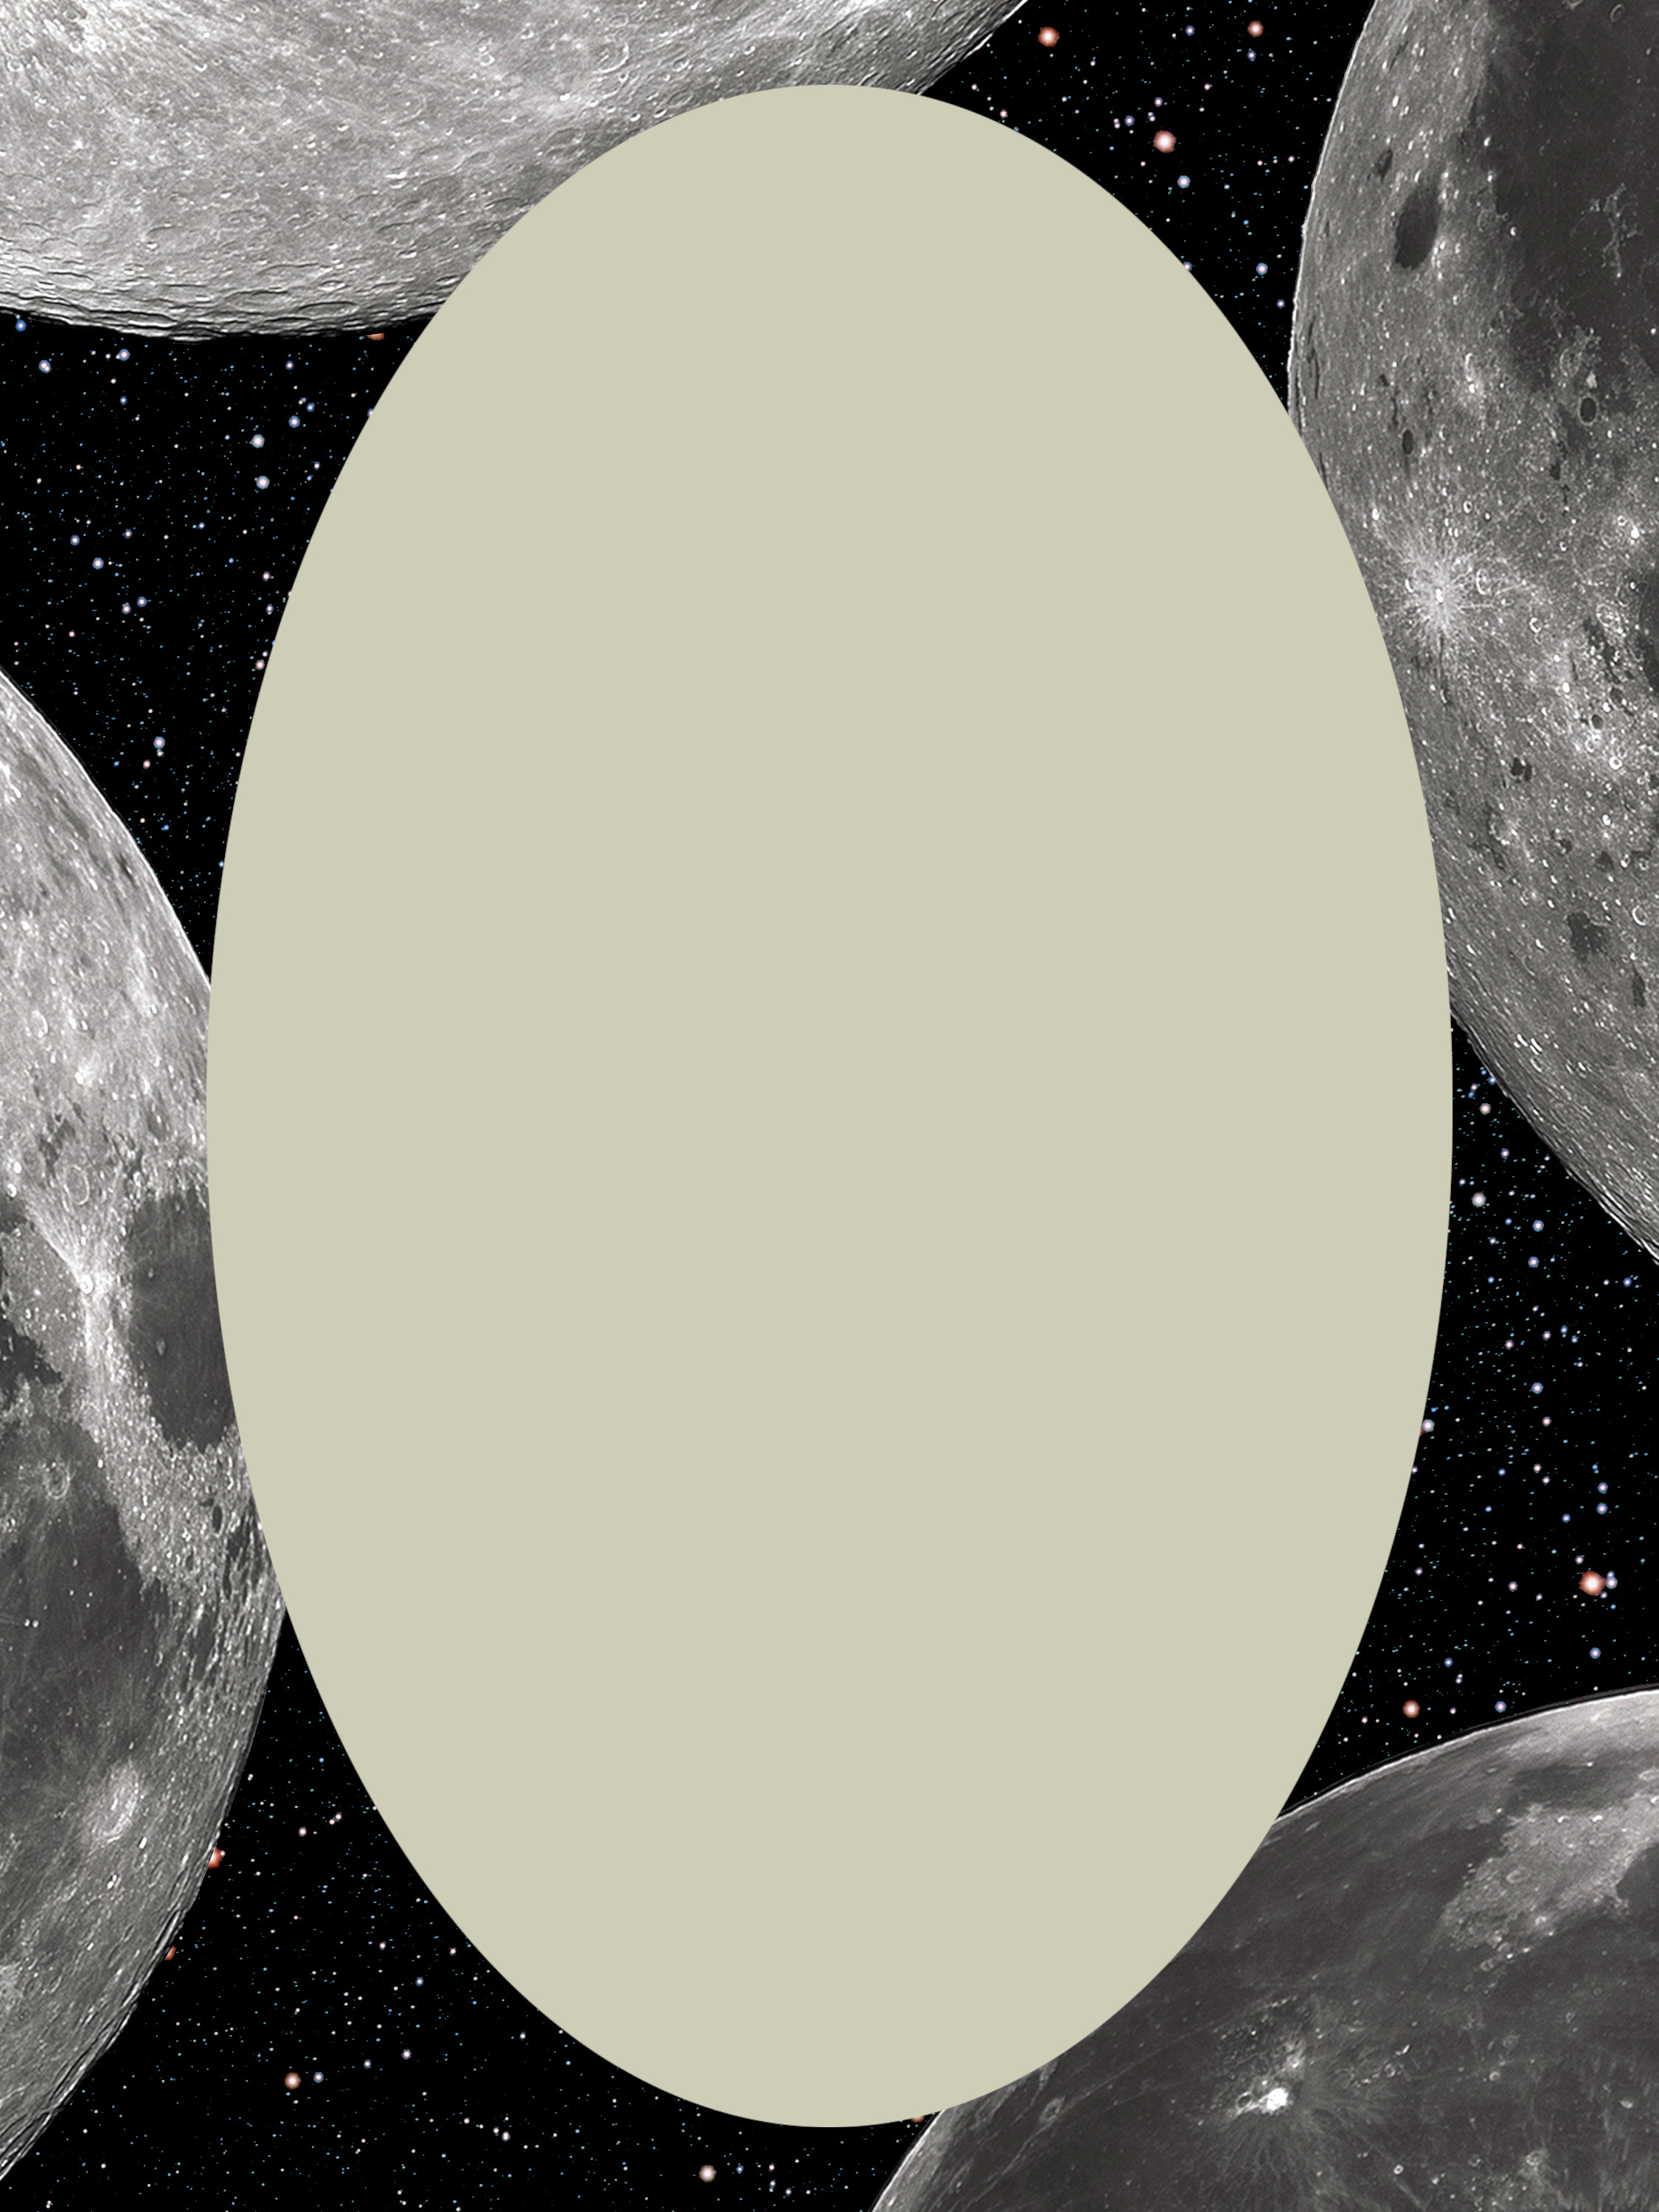
\includegraphics[width=\paperwidth,height=\paperheight]{moon-mist-large.jpeg}}
\begin{titlepage} % Suppresses headers and footers on the title page
	\centering % Centre everything on the title page
	%\scshape % Use small caps for all text on the title page

	%------------------------------------------------
	%	Title
	%------------------------------------------------

	\rule{\textwidth}{1.6pt}\vspace*{-\baselineskip}\vspace*{2pt} % Thick horizontal rule
	\rule{\textwidth}{0.4pt} % Thin horizontal rule
	
	\vspace{1\baselineskip} % Whitespace above the title
	
	{\scshape\Huge Somnium}
	
	\vspace{1\baselineskip} % Whitespace above the title

	\rule{\textwidth}{0.4pt}\vspace*{-\baselineskip}\vspace{3.2pt} % Thin horizontal rule
	\rule{\textwidth}{1.6pt} % Thick horizontal rule
	
	\vspace{1\baselineskip} % Whitespace after the title block
	
	%------------------------------------------------
	%	Subtitle
	%------------------------------------------------
	
	{\scshape \Large Joannis Keppleri\\\large Mathematici olim imperatorii }
 
        \vspace{0.5\baselineskip}

        {\scshape \normalsize \emph{Seu} Opus Posthumum de Astronomia Lunari}

        \vspace{0.5\baselineskip}
        
        {\scshape \small \emph{Divulgatum}\\ \emph{à} \\M. Ludovico Kepplero Filio\\ Medicinæ Candidato} % Subtitle or further description
	
	\vspace*{1\baselineskip} % Whitespace under the subtitle
	
        {\scshape \normalsize } % Subtitle or further description

	%------------------------------------------------
	%	Editor(s)
	%------------------------------------------------
        \vspace*{\fill}

        \begin{figure}[H]
        \centering
        \includegraphics[width=0.2\textwidth,keepaspectratio]{006-trans.png}
        \end{figure}

	\vspace{1\baselineskip}

	{\small\scshape Anno 1634}
	
	{\small\scshape{Impressum partim Sagani Silesiorum, absolutum Francofurti, sumptibus hæredum authoris}}
	
	\vspace{0.5\baselineskip} % Whitespace after the title block

        \scshape Internet Archive Online Edition% Publication year
    
	{\scshape\small Namensnennung Nicht-kommerziell Weitergabe unter gleichen Bedingungen 4.0 International} % Publisher
\end{titlepage}
\setlength{\parskip}{1mm plus1mm minus1mm}
\clearpage
\begin{figure}[H]
\centering
\includegraphics[width=0.95\textwidth,keepaspectratio]{002-trans.png}
\end{figure}
\begin{center}
Illustrissimo Celsissimoque

\emph{Principi ac Domino}

\textbf{Dn. Philippo, Landgravio}

{\small Hassiæ, Comiti in Catzenellenbogen, Dietz, Ziegenhaim et Nittau, etc. Dn. ac Principi suo Clementissimo, etc.}
\end{center}
\paragraph{}
\emph{Cum Illustrissime Celsissimeque Princeps, Domine Clementissime, Pater meus} Johannes Kepplerus Mathematicus Cæsareus, \emph{iam satis esset de fatigatus à motu molis terrestris, somniare cœpit de Astronomia et motu corporis Lunaris, sed nescio quid ominis secum at tulerit hoc somnium! Nobis sanè suis liberis luctuosissimum; licet ipsi fuerit satis delectabilis, imò exoptatissimus huius ominis eventus. Conscriptum n. hoc Somnium, cùm sub prælo versaretur, somno, (proh dolor!) captus Pater graviori, imò lætali, spiritu supra Lunarem regionem ad æthera (uti speramus) evolavit, nos liberos Martis iniuriis et Mundi huius miseriis expositos, omnique ferè temporali ope destitutos deseruit. Huius impressionis curam, cum Vir Clariss. atque Doctiss. Dn.} Jac. Bartschius \emph{Med. Doct. et Matheseos in Academiâ Argentinensi Professor designatus, affinis meus, suscepisset, re nondum confectâ ipse quoque morbo correptus læthali obiit.}

\emph{Ego interim à peregrinatione, quam cum Barone quodam Austriaco susceperam, in Germaniam reversus, indè à biennio nullam habens notitiam conditionis meorum, Francofurto in Lusatiam ad ipsos scripsi, ut quomodo et an vivant, me certiorem facerent; Et ecce Noverca vidua cum quatuor pupillis ære destituta ad me venit. Et quidem in statu turbulentissimo, inque locum propter annonæ charitætem inconvenientissimum, post se ducens exemplaria huius Somnii incompleta, opemque meam implorans, qui ipse aliorum auxilio et promotione opus habeo. Completionem item exemplarium huius Somnii à me postulat: sed quid ego boni sperare de hoc Somnio potero, cum Patri et affini fuerit lethale? Interim tamen, cum nomen Parentis adeò clarum et honorificum non occultare; sed potiùs, si ingenio suo famam augere non possit, tamen conservare pro viribus, filium deceat, Ego quoque petitionem hanc recusare non potui, imò affectavi. Sed Patronus huic operi adhuc deest. Certè inter militares unus vix reperietur, ut qui parum iam sunt solliciti de globi Lunaris Astronomiâ, quin potiùs circumspicere coguntur, ne à globis sclopedariis et tormentariis contundantur aut lædantur. Quare digniorem Te, Illustrissime Princeps, cuius patrocinio hoc opusculum frui possit, haud invenire potui, Ut qui ipse en studio Mathematico es exercitatissimus: qui à furore bellico es alienissimus: quique patrocinio tuo Clementissimo, Parentem nostrum, dum adhuc in vivus esset, fovebas. Quare Pupilli firmâ fiduciâ freti, Te, et ipsis et opusculo huic, Patrocinium Tuum non esse denegaturum. Illustriss. Celsit. Tuæ, per me, sese et Somnium hoc humiliter commendant, Deum Opt: Max: ardentissimis precibus exorantes, ut Illustriss. Celsit. Tuam cum Coniuge Illustrissimâ, secundum corporis et animæ vires diu conservare, et omnem hostilem impetum atque molestias militares à ditione ipsius avertere, clementer dignetur.}

\bigskip

\emph{Tuitaque Celsiss. Princeps Deo et Patriæ diutissime Vale. Dabam Francofurti ad Mœnum, die 18. Sept. An. 1634.}

\begin{center}
Illustriss. Celsit. Tuæ

\emph{Addictissimus}

\textbf{M. Ludovicus Kepplerus}

Medicinæ Candidatus.
\end{center}
\clearpage
\begin{figure}[H]
\centering
\includegraphics[width=0.95\textwidth,keepaspectratio]{001-trans.png}
\end{figure}
\section{Somnium, sivè Astronomia Lunaris}
\paragraph{}
Cum Anno 1608. serverent dissidia inter fratres Imp. Rudolphum et Matthiam Archiducem; eorumque actiones vulgo ad exempla referrent, ex historia Bohemica petita; ego publica vulgi curiositate excitus, ad Bohemica legenda animum appuli. Cumque incidissem in historiam Libussæ Viraginis, arte Magica celebratissimæ: factum quadam nocte, ut post contemplationem siderum et Lunæ, lecto compositus, altius obdormiscerem: atque mihi per somnum visus sum librum ex Nundinis allatum perlegere, cuius hic erat tenor.

\emph{Mihi\footnote{Notæ, successivè scriptæ inter annos 1620. 1630. Sonus ipse vocis mihi occurrit ex recordatione Nominum propriorum similiter sonantium historiæ Scoticæ, quæ regio prospectat Oceanum Islandicum.} Duracoto\footnote{Lingua nostra Teutonica sonat Terram glacialem. In hac verò remota insula locum ego mihi dispexi dormiendi et somniandi; ut imitarer Philosophos in hoc genere scriptionis. Nam et Cicero trajecit in Africam somniaturus, et Plato Atlanticam in eode Oceano Hesperio fabricatus est, unde fabulosa virtuti militari subsidia accerseret, et Plutarchus denique, libello de facie Lunæ: post multum sermonem in Oceanum Americanum exspaciatur, describit\'que nobis situm talem insularum, quem Geographus aliquis modernus Azoribus, et Gronlandiæ et Terræ Laboratoris regionibus circum Islandiam sitis probabiliter applicaverit. Quem quidem Plutarchi librum quoties relego, toties impensè soleo mirari, quo casu factum sit, ut nostra nobis somnia seu fabulæ tam accuratè congruerent. Nam ego quidem sat fidâ memoriâ repeto occasiones singularum commenti mei partium; quòd eæ mihi non omnes sint natæ ex lectione hujus libri. Extat apud me charta pervetus, tuâ Clarissime D. Christophore Besolde manu exatata; cùm theses circiter viginti, de cœlestibus apparentijs in Luna, ex meis dissertationibus anno 1593. concepisses, eas\'que D. Vito Millero tunc disputationum Philosophicarum ordinario Præsidi, disputaturus de ijs, si ipse annuisset, exhibuisses. Quo quidem tempore Plutarchi opera mihi nondum visa erant. Posteà incidi in Luciani libros duos historæ veræ, græcè scriptos: quos ego libellos mihi delegi, ut linguam addiscerem, adjutus jucunditate audacissimæ fabulæ, quæ tamem aliquid de totius universi natura innuebat; ut quidem ipse Lucianus monet in exordio. Atque etiam ille ultra columnas Herculis in Oceanum enavigat, rapitur\'que ventorum turbinibus cum ipsa navi sublimis, et Lunæ invehitur. Hæc mihi prima fuêre vestigia itineris in Lunam posterioribus temporibus affectati: Grætij primùm anno 1595. Plutarchi libellum sum nactus, admonitus de eo, ex lectione Commentarij Erasmi Reinholdi in Theorias Purbachij; ex\'que eo Pragæ anno 1604. multa in Astronomiæ partem opticam transtuli. Non dedi tamen hoc insulis à Plutarcho nominatis ex Oceano Islandico, quòd Islandiam ad Hypothesin mei somnij elegi. Sed erat hæc inter causas, quòd id temporis Pragæ venalis esset libellus Luciani de navigatione in Lunam, translatus in linguam Teutonicam à Rollenhagij filio, junctis narrationibus, S. Brandani, et de Purgatorio Patriciano in subterraneis Islandici montis Heclæ ignivomi: cùm etiam Plutarchus ex sententia Theologiæ gentilium, purgatorium animarum statueret in Luna; placuit mihi, profecturo in Lunam, potissimùm ex Islandia solvere. Major hujus insulæ commendatio fuit à narratione Tychonis Brahei, de qua infrà. Nec nihil potuit recordatio lectionis historiæ de Hibernatione Hollandorum in glaciali nova Sembla, quæ et ipsa plurima præbet exercitia Astronomica à me translata in Astronomiæ partem Opticam anno 1604.} nomen est, patria Islandia, quam veteres Thulen dixêre\footnote{In habitatione mea, quâ utebar ex concessione Martini Bacchatij, Rectoris Academiæ Carolinæ, pendebat ad parietem Charta Geographica Europæ pervetus, in qua vocabulum \textbf{Fiolx} Islandiæ locis adscriptum erat. Id quicquid sonaret, placuit milhi truci sono; addidi\'que usitatum fœminis in veteri lingua vocabulum \textbf{Hildis}; unde \emph{Brunhildis, Mathildis, Hildegard, Hiltrud} et similia.}: mater erat Fiolxhildis, quæ\footnote{Quia verisimilius hoc de filio, matris artium promulgatore, quam si eâ superstite scribere fingeretur. Sed et hoc innuere volebam, Imperitâ experientiâ, seu medicorum usu loquendi, Empiricâ exercitatione genitrice, nasci prolem Scientiam: atque illi non tutum esse, quamdiu superest inter homines mater Ignorantia, rerum causas occultissimas in vulgus propalare; quin potiùs parcendum verecundiæ antiquitatis, expectandam annorum maturitatem, qua veluti senio confecta Ignorantia, tandem emoriatur. Cùm igitur Somnij mei scopus sit, argumentum pro motu Terræ, seu solutionem potius objectionum ab universali contradictione gentis humanæ desumptarum, moliri exemplo Lunæ: jam tunc extinctam satis arbitrabar, ex\'que memoria ingeniosorum hominum eradicatam veterem hanc Ignorantiam; etsi quidem luctatur etiamnum Anima in nexu artuum tam multorum, tot sæculis firmissimè coalito; superest\'que in Academijs annosa mater; sed ita vivit, ut mors ei vitâ fœlicior æstimanda videatur.} nuper mortua, scribendi mihi peperit licentiam, cujus rei cupiditate pridem arsi.\footnote{[...?]} Dum viveret, hoc diligenter egit, ne scriberem. Dicebat enim, multos esse perniciosos osores artium,\footnote{Id mihi in peregrinatione mea nupera sic evenit; quanquam non soli, sed cœtui plurium consentientium. Cùm enim nos Theologus, Augustanam Confessionem professus, ingenti cum zelo invasisset, ex\'que Scriptura sibi videretur machinas petere ad nos oppugnandos; tandem accensus nostris defensionibus sublatâ voce, contestatus\'que omnia sacra, dogma hoc \emph{contra omnem rationem} pugnare exclamavit. Cùm ego, rupto denique silentio contumaci, hactenus enim assederam auditor merus, \emph{Nimirum}, inquam, \emph{hoc est, quod vestræ factionis homines urget vel ignaros. Si enim dogmatis hujus utilitatem, necessitatem et possibilitatem} rationis vestræ \emph{angustiis caperetis, jamdudum vim argumentorum à Scriptura petitorum vos ipsi declinaretis, quæsitâ commodâ interpretatione, ut aliàs soletis non rarò. At nunc tanta est rationis tuæ imbecillitas, ut non videas, etiam penes nos particulam aliquam esse rationis. Non igitur} contra omnem rationem \emph{dogma pugnat}; \emph{quod contra Astronomorum et Physicorum rationem non pugnat. Quod enim non capit unus, capit alter in materia peritior.}} qui quod præ hebetudine mentis non capiunt, id calumnientur\footnote{Sua cuique injuria, in Copernici opus Revolutionum hæc capitalis est injuria, quòd imperiti rerum Astronomicarum (Censuras librorum non ex mente sua, sed perperam interpretati) existimant, non esse legendum id opus, nisi prius exempto motu Terræ: quod tantundem est, ac si diceres, non legendum esse prius, quàm flammis fuerit exustum. Hos itaque non argumentis ego, sed risu refutandos ratus, tale scripsi Epigramma:\\\hspace*{5mm}Ne lasciviret, poterant castrare Poetam,\\\hspace*{5mm}Testiculis demptis vita superstes erat.\\\hspace*{5mm}Væ tibi Pythagora, Cerebro qui ferris abusus;\\\hspace*{5mm}Vitam concedunt, ante sed excerebrant.}: legesque figant injuriosas humano generi\footnote{Fallor an author Satyræ procacis, cui nomen Conclave Ignatianum, exemplar nactus erat hujus opusculi; pungit enim me nominatim etiam in ipso principio. Nam in progressu miserum Copernicum adducit ad Plutonis tribunal, ad quod, ni fallor, aditus est per Heclæ voragines. 3. 5. 8. 9. Vos amici, qui notitiam habetis rerum mearum, et quæ mihi causa fuerit peregrinationis proximæ in Sueviam, præsertim, si qui vestrum antehac manuscriptum nacti fuerunt, libellum istum, ominosa ista mihi meis\'que fuisse censebitis. Nec ego dissentio. Magnum equidem est mortis omen in vulnere lethali inflicto, in veneno epoto: nec minus fuisse videtur cladis domesticæ, in propalatione hujus scripti. Credideris scintillam delapsam in materiam aridam: hoc est, exceptas voces istas ab animis intus furvis, furva omnia suspicantibus. Primum quidem exemplar Praga Lipsiam, inde Tubingam perlatum est anno 1611. à Barone à Volckerstorff, ejus\'que morum et studiorum Magistris. Quantùm abest, ut credatis, in Tonstrinis, (præsertim si quibus est ab occupatione Fiolxhildis meæ nomen ominosum) in his igitur, confabulatum fuisse de hac mea fabula? Certè equidem ex illa ipsa urbe et domo enati sunt sermones de me ipso calumniosi proximè succedentibus annis: qui excepti ab animis insensis, tandem exarserunt in famam, imperitiâ et superstitione sufflantibus. Nisi fallor, sic censebitis potuisse et domum meam carere vexatione sexennali, et me peregrinatione annali proxima, nisi sominiata præcepta Fiolxhildis hjus violassem. Placuit igitur milhi, somnium hoc meum ulcisci de negocio exhibito, vulgatione libelli: adversarijs aliud mercedis erit.}; quibus sanè legibus non pauci damnati,\footnote{Heclæ, montis ignivomi, nota est historia ex Mappis et libris Geographicis. In genere supplicij, respexi ad fabulam, ut existimo, Empedoclis illius, apud Diogenem Laertium, qui cùm Aethnam montem ascendisset, ut divinis post obitum potiretur honoribus, in ipsos se Crateras demisisse, se\'que flammis immolasse vivuus fingitur; qui fortassis causas æterni quæsiturus incendij, cæca\'que temeritate progressus eò, unde regredi non poterat; fatiscente sub vestigijs cinerum incrustata superficie; serâ pœnitudine curiositatis, nec ullâ famæ hujus curâ, lugentem invitus dimisit animam. Nam affine fatum C. Plinio fuit, qui Vesuviani clade incendij per infestos cinerum et pumicum imbres philosophandi causâ Pompejanum invectus, sulphureo fœtore et cineribus oppletis spiraculis suffocats est. Sic Homerus ænigmate Piscatorum, Aristoteles Euripi reciprocationibus excruciati vitam in undas abjecisse fabulosis narrationibus feruntur. Ita plerique amorem in se scientiæ ulciscuntur paupertate, et odijs ignorantum divitum provocatis.} Heclæ voraginibus fuerint absorpti.\footnote{Allusi ad mores barbaros idiotarum. Si etiam scientiæ matrem des, quam ego suprâ dixi, ignorantiam; Rationem verò patrem: equidem hunc patrem ab illa matre vel ignorari, vel celari par est.} Quod nomen esset patri meo, ipsa nunquam dixit,\footnote{In historica descriptione Scotiæ et Orcadum, authore Buchanano, mentio fit piscatoris, qui cùm esset annorum 150, ex juvencula uxore pater sit factus aliquot liberorum.} piscatorem fuisse, et centum quinquaginta annorum senem, decessisse perhibebat, me tertium ætatis annum agente, cùm ille septuagesimum plus minus annum in suo vixisset matrimonio.}

\emph{Primis pueritiæ annis mater me manu trahens, interdumque humeris sublevans, crebrò adducere est solita\footnote{Quia superius nives et confragosa, in summo ignes è subterraneis, ut testantur historiæ.} in humiliora juga, montis Heclæ,\footnote{Quia Islandia sub Polari circulo est sita. Sic audivi etiam à Tychone Brahe, qui hæc ex relatu recensuit Episcopi Islandici.} præsertim circa festum divi Joannis, quando Sol totis 24. horis conspicuus, nocti nullum relinquit locum.\footnote{Medicinæ et Astronomiæ studia cognata, ex eodem fonte, desiderio cognitionis rerum Naturalium. Herbariæ verò Empiricæ plerunque sunt annexæ superstitiones.} Ipsa herbas nonnullas legens multis cæremoniis, domique coquens,\footnote{Trita est hæc traditio, vera an falsa, in Geographicis, Gubernatores navium ex Islandia navigantes, Ventorum quem velint, aperto Venti utre excire: quod si quis ad Rosæ nauticæ Rhombos, indicu lum\'que magneticum, et rectionem gubernaculi transferat, is vera propemodum dixerit. Cùm enim 32. venti censeantur; quocunque ex 16 unius Hemisphærij flante, si gubernatoria peritia accesserit, indicio rosæ et remigio gubernaculi navis impelletur destinato ejus Hemisphærij itinere: ventos verò contrarij Hemisphærij dispaciando ad latera rursum prorsum\'que, quod appellant \emph{Lavare}, tantisper eludunt, dum ij in eorum contrarij Hemisphærij unum commutentur.} sacculos factitabat ex pellibus caprinis, quos inflatos ad vicinum portum venum importans pro Navium patronis, victum hoc pacto sustentabat.}

\emph{Cùm aliquando per curiositatem rescisso sacculo, quem mater ignara vendebat, herbis\'que et\footnote{Ita referebat Episcopus Islandicus Tychoni Braheo, Virgines Islandicas inter audiendum in Templo Verbum Dei, solere dicta aut voces nonnullas exceptas acu et filis coloratis admirabili celeritate in linteis exprimerenendo.} linteis, quæ acu picta, varios præferebant characteres, explicatis, ipsam hoc lucello fraudassem: mater irâ succensa, me loco sacculi Nauclero proprium addixit, ut ipsa pecuniam retineret. Atque is postridiè ex insperato solvens è portu, secundo vento\footnote{Scotiâ et Orcadibus superiori Oceano præteritis.} quasi Bergas Nordwegiæ tendebat. Post aliquot dies\footnote{Scilicet hic sacculo caruit, ut Boreæ injurias effugere, Nordwegiam destinatam attingere non posset.} Boreâ surgente, inter Nordwegiam et Angliam delatus, Daniam petijt, fretum\'que emensus, cùm haberet literas\footnote{Ex relatu Tychonis, ut suprà N. 13.} Episcopi Islandici, tradendas Tychoni Brahe Dano; qui in Insula Wena habitabat, ego verò vehementer ægrotarem ex jactatione\footnote{De Rangiferis, cervorum Septentrionalium genere, scribit ad Landgravium Hassiæ Tycho Braheus, eos non durare in Dania, quòd illa quantumvis frigida regio, multò tamen sit tepidior Boddiâ, Finnoniâ, Lappiâ, ubi nascitur hoc animal. Islandiæ igitur, quæ et ipsa sub Arctico Polari sita, eandem frigoris magnitudinem tribuere consentaneum est.} et auræ tepore insueto, quippè quatuordecim aunorum adolescens: navi ad littus appulsa\footnote{Nullos habet incolas illa insula, quippe sterilis et saxosa, nec ampla præter piscatores ad 40.} me apud piscatorem insulanum exposuit cum literis; et spe reditus factâ, solvit.}\footnote{Hic viti verè philosophici mos fuit perpetuus, percontari, discere, magni facere narrationes hujusmodi, crebrò ruminare, ad theoremata physica applicare.}

\emph{Literis traditis Braheus valdè exhilaratus, cepit ex me multa quærere\footnote{Idem quidem Teutonismus, diversissimæ verò ejus dialecti in Dania, in\'que Islandia, quæ, ut apparet, Nordwegiorum est colonia: ad quos ejus et vicinæ Gronlandiæ Imperium ante centum annos pertinuit. Quin etiam Orcadas ipsas Teutonum mores et linguam obtinuisse ante 200 annos, ex narrationibus cujusdam mercatoris Veneti naufragi constat.}; quæ ego linguæ imperitus non intellexi, paucis verbis exceptis. Itaque negocium suis dedit Studiosis,\footnote{Rarò infrà decem, nonnunquam ad triginta: quos exercere solitus est tractatione instrumentorum variorum, ad observationes siderum; descriptionibus, computationibus, Pyronomicis laboribus, et similibus Philosophiæ studijs.} quos magno numero alebat, uti mecum crebrò loquerentur, factum\'que\footnote{Opum suarum, quæ magnæ ei erant ex hæreditate, dominus erat, largus\'que in studia dispensator: victor insuper omnis tædij, rerum\'que vulgò desperatarum affectator indefessus: quod observandi ratio accuratissima demonstrat; in qua cum ipsa Natura visus humani pugnavit, vicit\'que.} liberalitate Brahei, et paucarum septimanarum exercitio, ut mediocriter Danicè loquerer. Nec minùs ego promptus in narrando, quàm, illi erant in quærendo. Multa quippè insueta mirabar, multa mirantibus ex mea patriâ nova recensebam.}

\emph{Denique reversus navis magister, meque repetens,\footnote{Fuit hæc inter delectationes ejus viri una, ut nonnunquam abituros ex insula, jam\'que dimissos, percelleret inopinatâ repulsâ apud cymbarios, teneret\'que ultrà quàm vellent; nisi quis volare didicisset.} repulsam tulit, valdè me gaudente.}

\emph{Mirum\footnote{[...?]} in modum mihi arridebant Astronomica exercitia; quippè Studiosi et Braheus, mirabilibus machinis totis noctibus intendebant Lunæ sideribusque, quæ me res admonebat matris, quippè\footnote{Versabar tunc in lectione Operis Martini Delrio de disquisitionibus magicis. Et notus ex Virgilio versus:\\\hspace*{5mm}Carmina vel cœlo possunt deducere Lunam.\\\hspace*{5mm}Ante omnia quadrabat plaga cœli: Nam in Islandia sæpè Luna, cæteris populis plena, non apparet: Et Septentrionalibus populis magiam familiarem tradunt scriptores, et credibile est spiritius illos tenebrarum insidiari longis illis noctibus: est verò et Islandia in Septentriones profundè recondita. Nimirum et Philosophiæ sunt amica sublustris lucis ocia, noctes\'que continuatæ. Confirmat Illustrissimus Wirtembergiæ Dux Julius Fridericus, qui peregrinatione memorabili Septentrionem quoque pervagatus, viros ait passim in eo reperiri ad miraculum doctos, et Philosophiam inusitatâ nobis humanitate erga advenas reddentes.} et ipsa assiduè cum Luna solita erat colloqui.}

\emph{Hac igitur occasione ego patria semibarbarus, conditione egentissimus, in divinissimæ scientiæ cognitionem veni: quæ mihi ad majora viam paravit.}

\emph{Etenim exactis annis aliquot in hac Insula, tandem me cupiditas incessit revisendæ patriæ; rebar enim non grave mihi futurum ob acquisitam scientiam; emergere ad aliquam in mea gente rudi digniatem. Salutato igitur patrono, et veniâ discessus impetratâ, veni Hafniam; nactusque socios itineris, qui me ob linguæ et regionis cognitionem libenter in suum patrocinium susceperunt: redij in patriam, quinto postquam excesseram anno.}

\emph{Prima mei reditus felicitas erat, quod matrem inveni adhuc spirantem, et eadem, quæ olim, factitentem; finemque ei pœnitudinis diuturnæ, ob amissum temeritate filium, vivus et ornatus attuli.\footnote{Hoc tempus anni commodissimum navigationi ex Portu illo regni Daniæ in Islandiam sum ratus.} Vergebat tunc annus in Autumnum,\footnote{Id sequitur ex Num. 13. per doctrinam sphæricam.} succedebantque deinceps noctes illæ nostræ longæ, quippè Natalitio Christi mense Sol in Meridie vix parum emergens, è vestigio rursum conditur.\footnote{Redi ad Notam 28.} Ita Mater per hanc vacationem à suis operis, mihi adhærere, à me non discedere, quocunque me cum commendatitijs literis recepissem; percontari jam de Terris, quas adijssem, jam de Cœlo, quam scientiam me didicisse vehementissimè gaudebat: comparare quæ ipsa habebat comperta, cum meis narratis, exclamare\footnote{Judicibus lites, aurigæ somnia currus,\\\hspace*{5mm}Quas\'que die quæris, nocte potiris opum.} jam se promptam esse ad moriendum, ut quæ scientiæ suæ, quam solam possideret, filium hæredem sit relictura.}

\emph{Ego naturâ cupidissimus perdiscendi nova, quæsivi vicissim ex ipsa, de suis artibus, et quos earum habuisset magistros in gente tantùm à cæteris diremta. Tunc illa quodam die, spacio ad loquendum sumpto, rem omnem à primis initiis repetijt, in hunc ferè modum? Prospectum est Duracote fili, non cæteris solùm provinciis, in quas venisti, sed nostræ etiam patriæ. Etsi enim nos urgent frigora et tenebræ, aliaque incommoda, quæ nunc demùm sentio, postquam ex te felicitatem intellexi regionum cæterarum\footnote{Perquam ingeniosos Islandos affirmavit Tychoni Brahe supradictus Episcopus.}: at nos ingenijs abundamus,\footnote{Spiritus hi sunt scientiæ, in quibus aperiuntur rerum causæ. Admonuit me hujus allegoriæ vox Græca Dæmon, quæ à δαΐειν deducitur, quod est Scire, quasi δαήμων. Hoc supposito lege jam notam 28. à § Nimirum.} nobis præstò sunt sapientissimi spiritus, qui tantam lucem regionum cæterarum, strepitumque hominum perosi, nostras appetunt umbras, et nobiscum familiariter conversantur. Sunt ex iis præcipui\footnote{Causa genuina numeri mihi excidit. An ad novem Musas respexi, quia et ipsæ Deæ sunt gentilibus, quod est mihi, spiritus? An has in numerum adscivi. 1. Metaphysica. 2. Physica. 3. Ethica. 4. Astronomia. 5. Astrologia. 6. Optica. 7. Musica. 8. Geometria. 9. Arithmetica?} Novem, ex quibus\footnote{Certus sum, hîc vel Uraniam è numero Musarum, vel Astronomiam è scientijs in animo mihi suisse. Quod nisi multis vitæ præsidijs carerent septentrionales, ob frigora; dicerem plus illos ad Astronomiam aptos esse quàm cæteros: quia dierum et noctium discrimina, res ad Astronomiam invitans, apud ipsos sunt majora.} unus mihi pecuariter notus, et vel\footnote{Si de Musis ista, vanitatis aliquid in cæteris arguitur. Sin de Scientijs, Physica docet etiam venena, procreat etiam Chymistas, incircumspecte tractata, Metaphysica præposterè affectata inflat, dogmata Catholica turbat subtilitatibus nimijs et importunis, Ethica magnificentiam commendat, non omnibus proficuam, Astrologia supertitionibus patrocinatur, Optica decipit, Musica famulatur amoribus, Geometria dominatui injusto, Arithmetica avaritiæ. Sed melior sensus, quòd cùm omnes seipsis sint mites et innoxiæ, (eo\'que non spiritus illi apostatæ et nequam, quibus est cum Magis et Sagis commercium, qui suæ crudelitatis et noxarum testimonium habent irrefutabile, à proprio suo patrono Porphyrio.) præcipuum tamen hoc sit in Astronomia, subjecti sui conditionibus.} maximè omnium mitis atque innoxius\footnote{Quærendo, quæ causa hujus numeri mihi fuerit, non plus profeci, quàm, quod totidem inveni literas, seu characteres in vocibus \textbf{Astronomia Copernicana}; quod\'que totidem sunt formæ conjunctionum inter binos Planetas, quorum sunt numero septem. Et jucundum hoc accedit, totidem etiam esse jactus binarum tesserarum Cubicarum. Est quippè 21 Numerus Trigonicus, basi 6. Allegoria Evocationis est ex Delrio et Magia desumpta; sub est autem sensus Grammaticus. \emph{Evocatur}, id est, \emph{enunciatur}.} viginti et uno characteribus evocatur.\footnote{Hoc etiam de Finnonibus Septentrionali gente, vicinis\'que Lappis commemorat Olaus et alij. Ego verò ad doctrinam traduxi de diebus naturalibus, Zonis et Climatibus, et ad experientiam Hollandorum in mari Glaciali, qui omnia sic comparata invenerunt, ut nos Astronomi hic foris jam à multis sæculis docendo scivimus.} Cujus ope non rarò momento temporis in alias oras, quas ipsi dixero, transportor,\footnote{Priora de plagis terrarum erant posita, quæ ab homine adiri possunt, hæc jam de cœlestibus regionibus accipite.} aut si ab aliquibus longinquitate absterreor, quærendo de iis,\footnote{Populare scomma est, credam potiùs, quàm ut in rem præsentem eam. Quærunt\'que plerique, dudúmne ex cœlo delapsi simus Astronomi? Quibus magis ad captum suum respondit Galilæi nuncius siderius: at validius est Rationis judicium, quæ testis est omni exceptione major; quod experti sunt Hollandi in illis suis Hibernis, Num. 39.} tantùm proficio, quantum si præsens ibi essem: qui pleraque eorum, quæ tu vel oculis notasti, vel fando accepisti, vel ex libris hausisti, eodem quo tu modo, mihi recensuit.}

\emph{Imprimis ejus, de qua toties mihi dixit, regionis, te velim spectatorem fieri, me comite: valdè enim mira sunt, quæ de ea narrat.\footnote{Luna Hebræis est Lbana, vel Levana, Selenitida potui indigetare; sed Hebrææ voces, remotiores ab auditu, majori superstitione commendantur in occultis artibus.} Levaniam indigitavit.}

\emph{Nec mora consentio, ut Magistrum illa suum accersat, et consideo, paratus ad audiendam totam et itineris rationem, et regionis descriptionem.\footnote{Ecce iterum, ut me necessitas ipsa meorum suppositorum ejecerit in hoc littus, quod Plutarchus legit, Saturni et ipse reditum in taurum commemorans. At series hujus electionis meæ talis fuit. Morem Astrologorum affectavi, ut tàm Solem, quàm Lunam in proprijs constituerem dignitatibus. Atqui Sol in Leone domicilio suo fuit, antequam Duracotus domum rediret: id si non fuisset, Sol quidem in eo signo, Luna in Cancro, domo itidem sua, collocari potuit, decrescens et corniculata: at incommodum hoc accessurum fuit, quòd Solem cogebar sub horizonte ortivo collocare: cùm nox congruentius eligatur ad ista. Propter hæc incommoda delevi signum Cancri, deserui\'que annum, quo Saturnus in Cancro fuit; annum sc. 1593, quo anno scripta fuit illa disputatio Lunaris, tuâ Besolde manu: quas lituras etiamnum invenio in primo meo exemplari. Vicissim igitur Duracoto meo exactâ hyeme in patria, Martium elegi, Solem\'que in æquinoctio, bono signo Astronomico, in\'que aditu Arietis exaltationis suæ: Luna igitur si corniculata debuit videri, in signo sc. Soli vicino: non equidem in alio dignitatem aliquam habuit, quàm in Tauro, exaltationem. Itaque ut videri posset juxta stellas alias, oportuit Solem sub occiduum horizontem referre, principio noctis, quod fuit ex voto, præsertim in signis longarum descensionum, in quibus Luna tali situ valde est conspicua toto corpore intra complexum cornu lucidi: ut in opticis, in\'que dissertatione cum nuncio siderio Galilæi denique in Epitoma dixi. Ut igitur etiam Saturnus Lunæ jungeretur, quod habent Astrologi argumentum occultarum artium; Saturnus quoque in Tauro ponendus fuit. Ita emergit tempus, quo maximè fervebant observationes Tychonis, anno 1589. TT/2T Mart versperi: quando etiam conjunctio in constellationem Pleiadum incidit, quod sidus juxta Lunam collocatum, imaginationes nati multiplicat, ut in Harmonicis concessi. Quin etiam Astronomicæ rationes commendant hunc asterismum in observatione Lunæ corniculatæ. Vide hujus generis Observationem in Opticis meis, Cap. 11. fol. 247. ex anno 1598. 8. April et 27 Julij.} Tempus jam erat vernum, Lunâ crescente in cornua, quæ ut primum Sole sub Horizontem condito cepit enitere, juncta Planetæ Saturno in Tauri signo; mater\footnote{Hæc quoque magica ceremonia: cui respondet in rarione docendi Astronomiam, quod ea nequaquam est professoria seu extemporanea, sed indiget omnis expedita responsio quiete, recollectione sensuum, conceptis\'que verbis. In particulari observationis cujusdam praxi, quæ mihi Pragæ circa illos annos crebra erat, quoties me convenerunt spectatores spectatricesve; solitus ego sum prius ab illis colloquentibus me subducere in angulum domus proximum, ad hoc opus electum, diei lucem excludere, senestellam aptare minutissimo ex foramine, parietem albo vestire; peractis ijs, advocare spectatores. Hæ mihi cæremoniæ, hi ritus; vultis et characteres? In tabella nigra, quæ mihi videbantur apta spectatoribus, cretâ perscripsi, literis capitalibus, literarum figurâ retrò versa (en ritum magicum) ut Hebraica scribuntur; hanc tabellam foris sub dio, situ literarum everso suspendi in Sole; ut ita quæ scripseram, ea introrsum ad album parietem pingerentur situ erecto, et si tabellam ventulus agitaret foris, literæ intus motu vago parietem reciprocarent.} seorsim à me se recipiens in\footnote{Qui supersunt ex dictis meis spectatoribus. videbunt, ubi quodnam id bivium fuerit, in habitatione mea recollegerint animis. At hîc jam Astronomicum intelligitur bivium in schemate cœlesti supposito, id\'que geminum, unum Solis in puncto æquinoctiali constituti; in quo se mutuò transcindunt æquator et Ecliptica Solis semita. Et extat im manuscriptis Braheanis eo die habita observatio alt. Solis in ipso puncto æquinoctiali. Alterum biuium est nodus Lunæ descendens, seu cauda Draconis, quæ tunc etat in fine Aquarij: ad quam respiciendum est Astronomo, ut sciat, quando Luna sit in limitibus; uti quidem tunc erat in Austrino limite, in fine Tauri; qui situs Lunæ invitat Astronomos ad observandam latitudinem limitum.} proximum bivium, et\footnote{Vide suprà Num. 44.} pauculis verbis, clamore sublato, enunciatis, quibus petitionem suam proponebat\footnote{Vide suprà Num. 44.}; cæremoniisque peractis, revertitur,\footnote{Hos quoque ludos ipsissimos adjicere sum solitus, tanto gratiores spectatoribus, quod intelligerent, ludos esse.} prætensâ dextræ manus palmâ silentium imperans, propterque me assidet. Vix\footnote{Hoc ipso ritu (hui quàm magicè magico) observaveramus paulò prius, quàm libellum ego conciperem, Eclipsin Solis, anno scilicet 1605. 2/T2. Octobris. Meministis qui interfuistis, Legati Palatini Neoburgici. In solario enim domus deliciariæ in hortis Cæsaris camerâ destituebamur obscurâ; quare pallijs obnubentes capita, ita diei lucem arcuimus.} capita vestibus (ut conventum erat) involveramus; cum ecce\footnote{Non impossibile existimo, varijs instrumentis singulas tàm vocales, quàm consonantes ad imitationem loquelæ humanæ repræsentare. Id tamen, quicquid futurum est, strepitui et screatui quàm vivæ voci similius erit. Et in hac mechanica puto nonnullas esse collocatas insidias superstitiosis et credulis, ut quandoque existiment, sibi loqui dæmonas, cùm præstigias magicas ars imitetur. Quanquam quid hujus verissimè contingat, id rectius alijs legitimè affirmantibus credo, quàm ipse nullâ propriâ suffultus experientiâ, negaverim.\\\hspace*{5mm}Offert se tamen hîc mihi jucunda memoria Matthiæ Seiffarti bonæ memoriæ Symmystæ à Tychone Braheo hæredibus suis relicti; qui tres menses insumpsit in computanda ex præceptis Tychonicis Ephemeride Lunæ in annum unum: cui equidem vox erat verbis hisce non absimilis, morbus etiam obtigit melancholicus et phreneticus, in quo non erat locus ludendi; qui\'que tandem in Hydropem lethalem exijt.} screatus exoritur blæsæ et obtusæ vocis; et statim in hunc modum, sed idiomate Islandico, insit.}

\subsection[Dæmon \emph{ex Levania}]{Dæmon\footnote{Scientia apparitionis siderum; à δαΐειν scire.} \emph{ex Levania}\footnote{Ex Luna accersita, in quam oculi per fictionem erant translati.}}
\paragraph{}
Quinquaginta\footnote{Uni gradui circuli magni in terræ globo adscribuntur 15 Milliaria Germanica. Ut quia Romæ est Alt. P. 41. 50. Noribergæ 49. 26, sub eodem ferè Meridiano, Milliaria igitur 114, et ad Danubij ripam 100. Rostochij A. P. 54. 10. Ergò Noriberga Rostochium 71. Sic Lincij A. P. 48. 16, Pragæ 50. 6. Differentia 1. 50. censentur verò milliaria 26. Si gradus unus habet milliaria 15, erunt in ejus circuli, hoc est, in orbis Terræ semidiametro Milliaria 860. Et verò in Hypparcho demonstro, et in Epit. Astr. Copern. à priori deduco, Lunam Apogæon 59 ferè semidiametris Terræ abesse. Ductis 59 in 860, producuntur 50740. milliaria.} millibus miliarium Germanicorum in ætheris profundo\footnote{Non sita est, sed natat potiùs, si ad Insulæ similitudinem respicimus. Sed hîc jam ad imaginationem visus loquendum fiuit. Nam qui in Luna esset, omninò is Lunam stare loco fixam existimaret.} sita est LEVANIA insula\footnote{Subest ratio physica, joco mixta, cur Eclipses Solis et Lunæ tantùm inferant malorum? Nimirùm mali spiritus, dicuntur potestates tenebrarum et aeris. Credideris igitur damnatos, et quasi relegatos esse in regiones umbrosas, in conum umbræ Terræ. Quando ergò hic conus umbræ Lunam attingit, tunc dæmones agminatim Lunam invadunt, umbræ cono pro scalis usi. Vicissim quando conus umbræ Lunæ Terram attingit, in Eclipsi Solis totali, dæmones per eum revertuntur in Terras, ut infrà. Num. 86. Hæ verò occasiones raræ sunt. Quatenùs verò hoc loco Dæmon sumitur pro scientia Astronomica: seria erit affirmatio, non aliud esse iter menti in Lunam, nisi per umbram Terræ, et quæ hinc dependent alia. Vide Sciametrian, Hipparchi partem.}: iter ad eam hinc, vel ex eâ in has terras rarissimè patet: et cùm patet\footnote{Si allegoriæ insistimus, facile est Rationi, adminiculo Sciametriæ, eniti ad cognitionem rerum cœlestium: sin de Natura corporum et Spirituum cogitamus; rursum patet ratio affirmati. Et indulgeo sanè hîc joco, fronte quidem in physicam ratiocinationem intenta; ad latera verò spiculis Satyricis passim evibratis in spectatores sui securos.} nostræ quidem genti facilè est\footnote{Hoc intellige physicè; si corpus, cui sua gravitas horæ spacio per 12 millia milliarium rapiatur in altum. Adde privationem aeris, de qua Num. 71, quâ homines perire necesse est, ut pisces privatione aquæ. Nam inter dogmata, quæ præstantissimis physicis accepta fero, hoc etiam est, Aeris superficiem cum ipsis montium altissimorum fastigijs, aut etiam inferius, terminari.}; hominibus verò transportandis planè difficilimum, et cum summo vitæ periculo conjunctum\footnote{Crebra occurrunt in scriptis Tychonis Brahei probra conjecta in hujusmodi homines, qui tamen Philosophiam jactant: dum ipse suos labores, vigilias\'que nocturnas comparat.}: Nulli à nobis sedentarij adsciscuntur in hunc comitatum, nulli corpulenti, nulli delicati\footnote{Respexi ad Epigramma, quo olim jocatus sum in habitum corporis Mæstlini præceptoris tunc mei. Quò levius gracili fert corpore pondus; Hoc citius superas evolat ille domos. Gracilitas ingenij, subtilis est nota. Interim ignoscite, qui estis puncti.}; sed legimus eos, qui ætatem veredorum assiduo usu consumunt, aut qui navibus frequenter Indias adeunt, pane biscocto, allio, piscibus duratis, et cibis abhorrentibus victitare sueti.\footnote{En Aulida, et fœdus, quod Trojam perdidit. Mihi verò tantum jocari, erat animus; et jocose argumentari. Si verum est, inquam, quod de Sagis tradunt pleraque tribunalia, quòd illæ transportentur per aerem: erit fortè et hoc possibile, ut corpus aliquod terris divulsum importetur in Lunam.} Inprimis nobis aptæ sunt vetulæ exsuccæ, quibus indè à pueritia trita est ratio, hircos nocturnos, aut furcas, aut trita pallia inequitandi, trajiciendique per immania terrarum spacia.\footnote{Est inter apparatus jocorum et hoc, ut dum applausum unius audiente altero captare censeris, ferias et hunc, et proximum. Laudem tamen habet, ut Germania corpulentiæ et edacitatis, sic Hispania ingenij et judicij, et frugalitatis. In subtilibius igitur scientijs, cujusmodi est Astronomia (et præsertim hæc Lunaris, constans positione insolenti, si quis ex Luna spectaret) si pariter annitantur Germanus et Hispanus, multum hic prævertet. Et libellum igitur hunc prædixi deridiculo futurum Germanis, at in aliquo censu, Hispanis.} Nulli è Germania viri apti sunt: Hispanorum sicca corpora non respuimus.

Totum\footnote{Duratio Eclipsis Lunæ centralis ab initio ad finem, Luminaribus in Apogæis suis constitutis, excurrit pauculis minutis ulterius. Est enim Parallaxis Solis 0$^{\prime}$. 59$^{\prime\prime}$. Lunæ 58$^{\prime}$. 22$^{\prime\prime}$, summa 59$^{\prime}$. 21$^{\prime\prime}$, semidiameter Solis 15. 0. Ergò semidiameter Umbræ 44. 21. Cui addita semidiameter Lunæ 15. 0; summam restituit 59$^{\prime}$. 21$^{\prime\prime}$. Horarius verò Lunæ verus 29. 44. Solis 2. 23. Lunæ à Sole 27. 21. cujus duplum pro horis duabus ablatum relinquit 4$^{\prime}$. 39$^{\prime\prime}$. Sed 4$^{\prime}$. 33$^{\prime\prime}$. 30$^{\prime\prime\prime}$ conficiuntur Minutis 10$^{\prime}$. Et residua 5$^{\prime\prime}$. 30$^{\prime\prime\prime}$, Secundis 12$^{\prime\prime}$. Itaque tota duratio fit Horarum 4°. 20$^{\prime}$. 25$^{\prime\prime}$: Hæc tamen prolixitas est rarissima. Igitur si corpus aliquod terris profectum, Lunæ inferendum est; illud equidem aut multos per dies in cono umbræ terræ sublime circumferri debet, ut ad momentum ingressus Lunæ in hunc conum, præstò sit: aut si hoc naturæ coporis valde adversum et inimicum est; totum iter à terra ad Lunam brevissimo illo tempore, quo Luna in cono umbræ versatur, transmittet. Suppetit et causa ex philosophia magnetica. Luna terris cognatum corpus est. Multis id adstruit Plutarchus, libello de facie Lunæ hîc adjuncto, in persona unius ex colloquentibus. Trahunt et Aristotelem in partes, interpretes ejus Arabes. Nisi fallor locum illum Lib. 2. de cœlo, f. 426. de quo in præfatione in lib. 4. Epitomes Astron. Copernicanæ, cap. 12. nobis inculcant. Sed documentum evidentissimum cognationis hujus est in fluxu et refluxu maris; de quo vide introductionem meam in commentaria de motibus stellæ Martis. Luna in vertice constituta Oceani Atlantici, Oceani Australis dicti, Oceani Eoi, Oceani Indici, attrahit aquas, terræ globo circumfusas; quâ prolectatione fit, ut aquæ undique properantes ad locum spaciosum, terrarum\'que continentibus non interclusum, qui Lunæ ad perpendiculum est subjectus, detegant littora. Interim verò dum sunt in itinere, Lunâ à vertice unius Oceani abeunte, agmen aquarum impingens in littus Occidentale, desertum\'que à tractrice causa, refunditur, littoribus\'que Orientalibus vicissim infunditur. In Harmonicis lib. 4. Cap. ult. deliberavi de causa insuper aliâ fluxus et refluxus Maris; quæ huic quidem connexa est. Sed ea, quam hîc tango, sufficit instituto præsenti. Nam si Dæmones non alibi nisi in cono umbræ versantur; illi verò corpus aliquod in sublime versus coni verticem rapere finguntur: certè nisi Luna simul adsit, conum perambulans, soli erunt, nullâ re adjuti, laborabunt, sudabunt, defetiscentur scilicet. At si Lunâ secundâ opus aggredientur, ea præsens in umbra, tractu magnetico corporis cognati, conatus eorum adjuvabit. Vide infra N. 78.} iter quantum est, quatuor ad summum horarum spacio absolvitur.\footnote{En verò causam aliam brevitatis temporis ad hanc transvectationem, non longioris duratione eclipsis, non à natura corporis, sed à mente vectatorum accersitam.} Neque enim nobis semper occupatissimis, anteà constat de tempore eundi, quàm Luna ab orientis partibus ceperit deficere: quæ ubi tota luxerit, nobis adhuc in itinere hærentibus: irrita redditur nostra profectio.\footnote{Tota periodus ad allegoriam pertinet. Cùm raræ sint Eclipses insignes et magnæ, raræ occasiones eas observandi, scientia Astronomica (spirituum unus.) non vulgò per Eclipses, innotescit: sed Philosophi sunt, qui scientias philosophicas omnes (spirituum sc. horum familiam) impensè colunt: illi inquam tempori defectuum Lunarium insidiantur: illi scalis hisce usi, audent ascensum in Lunam, seu indagationem naturæ et cursus siderum affectare. Ex gente humana minima pars est eorum, qui philosophantur: è Philosophorum numero, vix unus est alter Astronomiæ fines proferre nititur.} Tàm præceps occasio efficit, ut paucos ex humana gente, nec alios, nisi nostri observantissimos comites habeamus.

Ergò\footnote{Revertor hîc ad contemplationem Naturæ corporum; fictione adhibitâ.} hominem aliquem hujus modi agminatim invadimus, omnes\'que subtus nitentes, in altum eum tollimus.\footnote{Gravitatem ego definio virtute, magneticæ simili, attractionis mutuæ. Hujus verò attractionis major vis est in coporibus inter se vicinis, quàm in remotis. Fortiùs igitur resistunt divulsioni unius ab altero, cùm adhuc sunt vicina invicem.} Prima quæque molitio durissima ipsi accidit.\footnote{Ictus validus non est, ubi facilè cedit corpus, quod truditur. Proptereà validiùs percutitur globus plumbeus, quàm lapideus, quia plus in illo ponderis, major igitur resistentia. Cum ergò corporea sint gravia, resistent motui: tàm pernicis igitur trusionis ictus violentissimus erit.} Nec enim aliter torquetur ac si pulvere Bombardico excussus, montes et maria tranaret.\footnote{Hîc ego doloris saltem acerbitati consului; caveat alius incolumitati viatoris, ne is minutatim contundatur, nullo discrimine dormiens, an vigilans.} Proptereà Narcoticis et Opiatis, statim in principio sopiendus est, et\footnote{In conglobatis, partes, proximæ causæ impellenti, plus patiuntur, pressæ pondere partium incumbentium.} membratim explicandus, ne corpus à podice, caput à corpore gestetur, sed ut violentia in singula membra dividatur.\footnote{Corpora nostra foventur tepore evaporationis continuæ ex visceribus terræ, quæ vel in pluvias, vel per noctem absente Solis radio calido, in rorem et pruinas coacta, decidit. Cutis, hoc tepido vapore extraneo denudata, horrere incipit. Vapor etiam ex corpore emanans, amisso calore, cujus vi expiraverat, in se coit, fit\'que jam materia frigida, et coagulationis operâ, motum acquirit versus corpus, undè pullulat; illatus\'que corpori, frigus illi infert. Aura denique ætherea, Solis radio destituta, frigida est, privatione caloris. Ea ut tenuissima, sic minimæ etiam efficaciæ frigus per se ipsa concipit, quamdiu immota est. At motus accedens, densitatis ei quandam vim effectu ipso conciliat, ut quo violentior impactus ejus in corpus, aut corporis volantis in ipsum, noc densior, et subtilitate suâ penetrantior, adeo\'que et frigidior fiat. Fit\'que frigus qualitas activa, densatione materiæ, quam nondum densatam privativè tantùm frigidam agnosco. Transitum à forma privativa ad activam, relinquo alijs explicandum. Vide speculationem hanc in Opticis meis, per comparationem lucis et coloris nigri, traductam; et quâ parte me vides laborare, adjuva ad causas eruendas.} Tunc excipit nova difficultas, ingens frigus, et\footnote{Vide suprà Num. 57.} prohibita respiratio,\footnote{Hoc tantùm dicis causa. Natura me deserit; ad jocum transire in re seria haud scio angratum. Allegoria etiam friget. Defectum rerum ad victum necessariarum, Dæmon ille, qui Astronomia dicitur, ingenitâ vi fervoris ignei ad speculandum, frigidè admodum supplet.} quorum illi, ingenita nobis vi,\footnote{Non erat prætereunda tàm opportuna narratio Aristotelis, de Philosophis in montem Asiæ Olympum speculationis causa connisis.} huic verò, spongijs humectis ad nares admotis, obviam imus.\footnote{Nimirùm ubi corpus ereptum ex orbe virtutis magneticæ telluris tanto spacio, ut jam præponderet virtus magnetica orbis Lunæ.} Confectâ primâ parte itineris, facilior redditur vectio.\footnote{Suspensis virtutibus magneticis Terræ et Lunæ contrariâ tractione; perinde est, ac si nullum corpus quoquam prolectaret. Tunc igitur corpus ipsum, ut totum, trahit sua membra, ut partes, minores toto.} Tunc libero aëri exponimus corpora, manus\'que subtrahimus. Atque illa in sese conglobantur ut aranei\footnote{Non planè nutu. Opus est viribus etiamnum. Nam omne corpus ratione materiæ suæ obtinet inertiam quandam ad motum, quæ corpori quietem præstat in omni loco, in quo id collocatur extra virtutes tractorias. Hanc vim, seu inertiam potiùs, necesse est vincat is, quid id corpus loco suo est emoturus.}: quæ nos solo ferè nutu transportamus,\footnote{Quando scil. ob propinquitatem, præpollet orbis virtutis magneticæ Lunæ. Posito enim, quod moles quælibet terræ, æqualis globo Lunari, trahat æquè validè; corpus sic locatum inter utrumque globum, ut eadem sit proportio suæ ab utroque distantiæ, quæ est ipsorum inter se corporum, hærebit immobile, tractionibus in diversa, se mutuò abolentibus: ut si absit à Terra 58 1/59 semidiametris Terræ, à Luna verò 58/59 partibus semidiametri terræ. Ideem verò paulò adhuc propiùs admotum Lunæ, jam Lunam trahentem sequetur, præpollente ejus vi ob propinquitatem.} adeò ut denique moles corporea sponte suâ vergat in locum propositum.\footnote{Initiò quidem parùm; at proximè Lunam valdè multùm, ut statim sequitur. Item; parùm utilis, planè nihil annitentibus: nitentes verò corpus tollere, etiam tum juvat, cùm adhuc terra præpollet: Vide suprà Num. 62.} Sed parum nobis est utilis hæc ῥοπὴ, quia nimis tarda: itaque nutu ut dixi acceleramus; et præcedimus jam corpus, ne durissimo impactu in Lunam, damni quid patiatur.

Solent\footnote{Vide Num. 67. 68. 69. Videat verò viator, ut sic incolumi corpore pervenerit, ut etiam expergisci possit. Allegoria hîc probatam medicinam propinat ijs, qui Virginitatis voto sunt obstricti, contra motus naturales; speculationem intentam, continuam, æstuantem.} homines, cum expergiscuntur, queri de ineffabili membrorum omnium lassitudine; à qua serò admodum se recipiunt, ut ambulent.

Multæ prætereà occurrunt difficultates, quas longum esset recensere.\footnote{Quod suprà Num. 6. corporum naturæ valdè adversum et inimicum; imò impossibile.} Nobis nihil admodum evenit mali. Tenebras enim Telluris quam longæ illæ sunt, confertim inhabitamus; quæ ubi LEVANIAM attigerint, præstò sumus,\footnote{Jucundissimum mihi, eadem penè verba me in Plutarcho jam invenire.} quasi ex navi in terram exscendentes\footnote{Quia spiritus tenebrarum dicuntur, ut suprâ Num. 55. Sed Allegoria, itineri per umbram, comparat Observationem Eclipsium; Soli, negocia politica; cavernis umbrosis Lunæ, secessum et umbras scholasticas; moræ in cavernis, speculationem continuatam, observationibus Eclipsium insistentem. Erat mihi Pragæ habitatio, in qua nullus angulus aptior observationi diametri Solis, quàm cella cerevisiaria subterranea; ex cujus fundo per foramen sublime, tubum Astronomicum in Opticis descriptum dirigere sum solitus in Solem meridianum diebus solistitialibus. Sed hanc partem Allegoriæ latius diducit numerus 83. seq.}: et ibi nos properè in speluncas et loca tenebrosa recipimus, ne nos Sol in aperto paulò pòst obruturus, optato diversorio ejiciat, umbram\'que discedentem insequi cogat.\footnote{[...?]} Dantur ibi nobis induciæ exercendorum ingeniorum ex animi sententia; conferimus cum ejus provinciæ dæmonibus, inita\'que societate,\footnote{Quod fit die 7 vel 8 post Eclipsin Lunæ, ut infrà.} ubi primùm locus Sole carere ceperit, junctis agminibus in umbram exspaciamur, et si illa mucrone suo,\footnote{Crebiores Solis, quàm Lunæ eveniunt totales defectus.} quod plerumque fit, Tellurem feriat,\footnote{Jocus supra Num. 55. explicatiùs propositus. Sed ad allegoriam si traxeris, elicies jam vicissim prædictiones Eclipsium Solarium, derivatas ex speculatione, quæ observationi deliquiorum Lunarium innititur.} Terris et nos, socijs exercitibus incumbimus: quod non aliàs nobis licet, quàm cum Solem homines viderint deficere. Hinc evenit, ut defectus Solis adeò metuantur.

Atque hæc de itinere in LEVANIAM dicta sunto.

Sequitur, ut de ipsius provinciæ forma dicam, exorsus, more Geographorum, ab ijs, quæ cœlitùs illi eveniunt.

Etsi\footnote{Si est enim ut semidiameter Solis ad semidiametrum orbis Saturni, sic hæc ad semidiametrum Fixarum, ut à priori deduxi Ep. Astr. Lib. 4: fit ut Saturnij cœli semidiameter vix sit bis millesima semidiametri Fixarum sphæræ; Cœli verò, in quo Terra cum Lunâ, vix vicies millesima; et Lunaris sphæræ semidiameter est pars 1/59 de semidiametro jam dicti cœli. Variantur igitur intervalla Telluris à fixis, parte non majore quàm est decies millesima; Lunæ verò digressiones adjiciunt hujus tam minutæ variationis particulam circiter tricesimam. Ita omnis Lunæ à fixis digressio efficitur planè insensibilis.} siderum fixorum aspectus tota Levania habet nobiscum eosdem; motus tamen Planetarum et quantitates, ab ijs, quas nos hîc videmus, observat diversissimas: adeò ut planè alia sit totius apud ipsos Astronomiæ ratio.

Quemadmodum\footnote{Quia Luna semper easdem maculas ad nos Telluris incolas convertit; ex eo intelligimus, illam circumire Terram, perindè ac si filo esset illi annexa; et parte sui superiore nunquam videre Terram, parte seu hemisphærio inferiori semper.} igitur Geographi nostri orbem terræ dividunt in quinque Zonas, propter Phœnomena Cœlestia\footnote{Quam nos Terram appellamus, Telluris incolæ: eam ex imaginatione populorum Lunarium libuit appellare Volvam. Quemadmodum enim nobis nocturnum Luminare Hebraicè \emph{Lebhana} dicitur à colore albicante, et dialecto Hetrusca (ex Punica, ut puto, derivatâ) \emph{Luna}; Græcè \emph{Selene} à σέλας, quod albicantem nitorem significat; quippè nobis in terra versantibus talis apparet: sic etiam populis Lunaribus, appellationem nostræ Telluris, quam illi loco alicujus Lunæ vident, ab apparitionis specie derivatam, tribui par est. Apparet verò ijs globus iste in cœlo, perpetuâ cum volutione circa suum axem immobilem, cujus volutionis indicium desumere illis licet à macularum varietate, ut infrà dicetur. A volvendo igitur Volva dicatur, et Subvolvæ vel Subvolvani, qui vident Volvam: Privolvæ, qui sunt privati conspectu Volvæ.}: Sic Levania ex duobus constat hemisphærijs, uno Subvolvarum, altero Privolvarum: quorum illud perpetuò fruitur suâ\footnote{Vide suprà Num. 89.} volvâ, quæ est illis vice nostræ Lunæ; hoc verò Volvæ conspectu in æternum privatur.

Et circulus Hemisphæria dividens, instar nostri coluri solstitiorum,\footnote{Nos in hoc Terræ globo, Polos mundi censemus, illa duo puncta sphæræ fixarum inter se opposita, in quæ axis Telluris utramque in plagam continuatus incidit. Hæc enim duo puncta in primi motus apparitione spectamus ut immobilia. Hæc duo puncta Lunaribus, poli Mundi non censentur: non apparet enim ipsis cœlum stellatum tam brevi temporis spacio, quod nos viginti quatuor horis nostratibus censemus, circa eos circumvolvi. At vicissim axis corporis lunaris, ad planum Eclipticæ rectus vel quasi, continuatus, incidit in puncta fixarum Polis Eclipticæ vicina: ij sunt Lunicolis poli Mundi; quia Sphæra fixarum spacio temporis, quod nos mensem dicimus, ijs circa hunc axem volvi cernitur, pro eo, quòd verè globus ipse Lunæ circa hunc suum axem, ejus\'que duas extremitates convertitur, velut immobiles loco. Etsi enim Globus Lunæ, et in eo, hic etiam axis, circa globum telluris menstruo spacio circumfertur; at manet ille interim in omni situ, sibi ipsi parallelus; eo\'que semper in una quidem revolutione eadem ferè puncta fixarum ostendit; quia orbis Lunæ amplitudo, comparata ad sphæram fixarum, fit insensibilis. Quod autem Divisor circulus, transeat per hos globi Lunaris polos, apparet ex eo, quia semper eædem maculæ Lunæ Telluri obvertuntur, toto tempore circuitus menstrui. Quantum enim de Lunæ globo nos ita cernimus velut immobile, tantum verissimè volvitur circa dicta puncta.} per polos munditransit, appellatur\'que Divisor.

Quæ igitur utrique sunt communia hemisphærio, primo loco explicabo.

Itaque\footnote{Quia globus Lunæ sic circumit circa Tellurem, ut semper idem hemisphærium ejus obvertatur telluri: quod possis anticam Globi hujus dicere: patet, eam, cùm inter Solem et Terram est, nobis\'que Nova seu exili cum cornu apparet, tunc tergum obvertere Soli, anticam à Sole avertere: at cùm nobis plena, interpositis sc. se inter et Solem: tergum obvertit fixis, à Sole avertens, anticam et Soli et Terræ objicit. Sol verò præsens diem, absens noctem efficere in toto mundo censetur. Habent igitur utrique suam diem et noctem, sed non tàm breve Νυχθήμερον, ut nos. Totum enim menstruum nobis spacium, ipsis absumitur in unius diei et noctis longitudinem.} Levania tota vicissitudines sentit diei et noctis, ut nos\footnote{Varietas dierum et noctium extra dies æquinoctiorum penes nos est ex eo, quod poli mundi longè nobis videntur distare à polis Eclipticæ. His quos nos habemus polis mundi, Lunares carent: contrà alios habent mundi polos, polis Eclipticæ proximos. Et si qua est varietas ex eorum distantia parvula à polis Eclipticæ, ea cum illa nostra comparanda non est; certè sensibilis adeò non est; eo\'que ferè perpetuum ipsi habent æquinoctium, per totum globum: sicut etiam penes nos in terra, die æquinoctij per totum orbem terrarum est æquinoctium.}: Sed carent illi hac nostrâ annuâ varietate toto anno. Per totam enim Levaniam æquantur dies ferè noctibus\footnote{In Ephemeridibus meis, phasis Lunæ bifalcata differt à quadratura Lunæ cum Sole ad summum duarum horarum nostratium spacio cum 10. Minutis: quod fit, quia proportio orbis Lunæ ad circuitum Solis (vel Terræ) est ut 1. ad 59, in Apogæo sc. Jam verò dies oritur Subvolvarum medijs, cum locus globi Lunæ constituitur in circulo illuminationis Lunæ, qui phasin format, non cùm in quadrato Solis versatur centrum globi Lunæ. Quare cùm in utrâque phasi fiat Luna propior Soli, quàm Terra; pars etiam orbitæ Lunæ ab his terminis exterius circa terram circumducta, longior est parte interius inter Terram et Solem continuatâ: Et illa pars exterior, medijs Subvolvarum admetitur diem, medijs Privolvarum noctem: Ergò Subvolvanis dies, Privolvis nox, præter tempus semimenstruum à nobis censitum, adsciscit insuper horas nostrates circiter quatuor; tantundem\'que nocti illorum, diei horum, vicissim decedit. Porrò quæ de medijs Hemisphæriorum sunt dicta, ea pertinent etiam ad succedentes versus ortum vel occasum, cum hac sola varietate, ut quot gradibus longitudinis quilibet locorum à Meditullio removetur, totidem etiam globus Lunæ superet situm illum, in quo Medijs dies oriebarur.}: nisi quòd Privolvis regulariter omnis dies est brevior suâ nocte; Subvolvis longior. Quid autem per circuitum annorum 8 varietur, infrà erit dicendum.\footnote{Sicuti fieri necesse est in globo terræ, sub ipso polo, die æquinoctij.} Sub utroque verò polorum, in compensationem noctis, Sol dimidius tegitur, dimidius lucet, montes circulo circumiens.\footnote{En hypothesin totius somnij, argumentum sc. pro motu Terræ, seu dissolutionem potiùs argumenti contra motum Terræ, ex sensu extucti.} Nec enim minùs Levania suis incolis immota stare videtur, currentibus astris, quàm Terra nostra nobis hominibus.\footnote{Si dies definitur præsentiâ Solis, præsens verò Sol est ibi, ubi loca ejus lumine cernuntur illuminata; certè totis 15 diebus eædem Lunæ maculæ in medio ejus corpore cernuntur à nobis illuminatæ continuè, nullâ interpositâ nocte, Lunâ enim plenâ, patet earum conspectus nobis, uno loco manentibus, ultra 16 horas; etiam\'que cum nobis Luna latet sub Horizonte, alijs apparet per rotunditatem Terræ. Dies igitur illorum est nostra Νυχθήμερα quindecim longa; et quod sequitur, nox illorum alia nostra quatuordecim et amplius.} Nox et dies juncti, æquant unum ex nostratibus mensibus: quippè Sole orituro manè, integrum ferè Zodiaci signum postridiè plus apparet, quàm pridie.\footnote{Si nos in terris, non populus quidem promiscuè, sed Astronomi tamem, numeramus in annis 8 menses 99; seu in annis 19, menses 235; quamvis Lunationes naturales negocijs nostris non eâdem necessitate immisceantur, quâ dies et noctes: quid aliud de Lunaribus populis, quos supponimus, cogitare possumus; quam eosdem illos observare numeros, si qua ibi creatura est, numeri capax; cùm aliam ipsi diem non habeant. Signum verò exactæ periodi 19 annorum, est ipsis, si eadem sidera pristino ordine exactè oriantur.} Et ut nobis in uno anno 365 Soles, et 366. sphæræ fixarum, seu præcisiùs in 4 annis 1461. Soles, sed 1465. sphæræ fixarum volvuntur: Sic illis in uno anno Sol duodecies, sphæra fixarum tredecies, seu præcisiùs in 8 annis Sol 99ies, sphæræ fixarum centies septies circumit. Sed familiarior est ipsis circulus annorum novendecim. Etenim in tot annis Sol oritur ducenties tricies quinquies, fixæ verò ducenties quinquagies quater.

Oritur Sol subvolvarum medijs seu intimis, quando nobis apparet ultima quadra, Privolvarum verò intimis tunc, quando nobis est prima quadra.\footnote{Medivolvanos intellige denominari ut nostros Meridianos. Sed nobis Meridiani plurimi sunt; ipsis Medivolvanus unicus, quippè per duo solum puncta hemisphæriorum, à Volva denominatorum, exactè invicem opposita. Non sunt tamen hi Medivolvani loco nostrorum Meridianorum: sed habent et Lunares, suos juxta Meridianos, per polos et vertices locorum ductos, socios quasi Medivolvani omnium medij. Nostri quidem Meridiani terrestres principium naturale non habent: illorum verò Meridiani habent, sc. medium omnium Medivolvanum; ut in quem Sol et Volva simul eodem momento incidunt, in Meridianos cæteros non eodem, sed distinctis.} Quæ autem de meditullijs dico, de totis semicirculis intelligenda sunt per polos et meditullia ductis, ad divisorem rectis: quos semicirculos Medivolvani appellare possis.

Est autem Circulus aliquis inter Polos intermedius, vicem gerens nostri æquatoris Terrestris: quo etiam nomine indigetabitur: bifariam secans tàm divisorem, quàm Medivolvanum in punctis oppositis: cui quæcunque loca subsunt: eorum verticem Sol quàm proximè quotidiè, et præcisè quidem diebus duobus oppositis in anno transit, in puncto meridiei. Cæteris qui versus polos utrinque habitant, in meridie\footnote{Cùm Luna globus sit, centrum ejus petent omnia gravia lunaria: et corpora, globi superficiei insistent ad angulos rectos; censebunt\'que hunc suum verticem inter fixas, in quem punctum recta ex centro globi lunaris per sua vestigia continuata incidit. Quæcunque stellæ ab illo puncto distant, à vertice observatoris in Lunâ collocati, declinare censebuntur. Hoc igitur est fundamentum imaginatonis Aequatoris inter polos medij et declinationis Solis a vertice locorum. Et quia ponitur Sol non quotidiè per totum annum transire verticem eorum, qui sub æquatore sunt; sed tantùm die æquinoctij: igitur axis globi Lunaris, circa quem ille convertitur, parallelus non est axi Eclipticæ, sed inclinatur ad eum: semper sc. ad rectos angulos erectus est super planum orbitæ Lunæ, quam illa quovis tempore permeat, ut inclinatâ eâ ad planum Eclipticæ, axis etiam illius ad axem hujus inclinetur.} Sol declinat à vertice.

Habent in LEVANIA et nonnullam vicissitudinem æstatis et hyemis: sed eam nec comparandam varietate cum nostra; nec ut nos, semper ijsdem in locis, eodem anni tempore.\footnote{Nodi Lunæ motu retrogrado circumeunt in annis 19, obviantes Soli; circumeunt igitur et limites eodem tempore, et poli orbitæ Lunæ, qui sunt Lunaribus loco polorum mundi, in circello, cujus diameter habet gradus 5. Annis igitur siderijs 19 conficiuntur apud ipsos anni Tropici 20. Itaque in 9 1/2 siderijs, hoc est in 10 Tropicis, decima æstas, ijs quibus initio contingebat, Sole in constellatione Cancri versante, contingit jam, Sole in Capricorni constellatione constituto. Tale quid etiam nobis in terra contingit, sed multò tardiùs. Nostra enim æstas ante duo millia annorum eveniebat, Sole in constellatione Cancri versante, cane cum Sole oriente; hodie profecta est nostra æstas in constellationem Geminorum: etsi dodecatemorium Zodiaci retinet nomen antiquum Cancri.} Fit enim decem annorum spacio, ut æstas illa migret ab una parte anni siderij, in partem oppositam, eodem loco supposito: quippè circulo annorum novemdecim sideriorum, seu dierum 235, versus polos vicies fit æstas, toties\'que hyems; sub æquatore quadragies: sunt\'que\footnote{Harum sex dierum una sola vel duæ sunt verè æstivæ, cæteræ ad latus utrumque, declinant ad quantitatem diei æquinoctialis.} apud illos quotannis sex dies æstivi, reliqui hyemales, ut apud nos Menses. Ea vicissitudo vix sentitur circa æquatorem, quia Sol non ultra 5 Gradum ijs locis rursum prorsum\'que ad latera vagatur. Magis sentitur juxta polos; quæ loca Solem alternis semestribus habent, aut nonhabent: uti penes nos in Terris, ij qui sub alterutro polorum habitant. Itaque etiam LEVANIAE globus in quinque Zonas abit; Terrestribus nostris quodammodò respondentes; sed Torrida vix habet 10. gradus, ut et Frigidæ; totum reliquum cedit\footnote{Temperatas enim et ipsas vix sustineo dicere. Nulla enim est in Luna temperies, ut apparebit.} temperatarum nostrarum Analogis. Et transit torrida per meditullia Hemisphæriorum: semissis scilicet longitudinis per Subvolvanos, reliquus semissis per Privolvas.

Ex\footnote{Zodiacum habent nobiscum communem. Noster enim Zodiacus motu annuo telluris circa Solem describitur: Luna verò et ipsa Tellurem nostram circumit, sicut nos eam circumhabitamus. Eadem igitur utrisque est causa imaginandi Zodiaci.} sectionibus circulorum æquatoris et Zodiaci existunt etiam quatuor puncta Cardinalia, ut sunt apud nos æquinoctia et solstitia: et ab ijs sectionibus, initium est Zodiaci circuli. Sed valdè velox est motus stellarum fixarum ab hoc initio in consequentia\footnote{Hæc sunt ijs correlata, quæ ad N. 101. sunt dicta Consentaneum enim est, respectum anni tropici, si non tantum, quantus est penes nos, majorem saltem esse penes Lunares, respectu sui anni tropici.\\\hspace*{5mm}Respice verò hîc ad Hypothesin libelli; et disce, quæ nobis sunt inter totius mundi præcipua; duodecim signa cœlestia, Solstitia, Aequinoctia, Annos Tropicos, Siderios, Aequatorem, Coluros, Tropicos, Polares, Polos Mundi; omnia restringi ad angustissimum globum Telluris, solâque Terricolarum imaginatione constare: ut si ad alium globum transferamus imaginationem, omnia mutata concipere necesse sit.}: quippè annis viginti Tropicis, id est, unâ æstate, et unâ hyeme definitis, totum Zodiacum transeunt, quod fit apud nos vix annis 26000.

Atque hæc de Motu primo.

Secundorum motuum ratio non minus est illis diversa ab ijs, quæ nobis apparent; multo\'que magis, quàm penes nos, intricata. Quippè omnibus Planetis sex, Saturno, Jovi, Marti, Soli, Veneri, Mercurio, præter tot inæqualitates, quæ sunt nobis cum illis communes, tres aliæ accidunt apud illos, duæ longitudinis, una diurna, altera per circuitum annorum 8 1/2: tertia latitudinis, per circuitum annorum 19.\footnote{Quia orbis Lunæ, seu distantia ejus à Terrâ apogæa, est 1/59 de distantia Solis et Terræ. Cùm ergò Privolvæ habent Solem in suo Meridiano, propiores Soli fiunt quàm terra, per 1/59 totius: at cùm Subvolvæ; remotiores. Luna quippe plena distat à Sole 60 partibus, Terra 59 Luna Nova 58. Cum diminutione verò intervalli, augetur Solis species. At in Quadris Luna existens, et Terra, æqualiter absunt à Sole. Et, in Quadris, diximus; Medijs tàm privolvarum, quàm subvolvarum, oriri vel occidere Solem.} Nam Medij Privolvarum Solem in meridie suo, cæteris paribus, habent majorem, Subvolvæ minorem quàm si is oriatur\footnote{Luna ab Ecliptica discedit ad latera circiter 5 gradus, ex terris inspecta; ex Sole verò, totidem circiter scrupula, quia orbium proportio est sexagecupla paulò major.}: utrique junctim existimant, Solem a liquot minutis ab Ecliptica rursum prorsum\'que declinare jam apud has, jam apud illas fixas; et hæc nutamenta, spacio 19. annorum, ut dixi, restituuntur in pristina vestigia.\footnote{Quando privolvæ Solem vident in suo meridie, Soli viciniores sunt Tellure; quando Subvolvani, remotiores; parte sexagesimâ paulò plus, et igitur Subvolvani Privolvis remotiores circiter tricesimâ totius. Itaque si Sol declinat Privolvis cum plurimùm, scrup. 5$^{\prime}$. 30$^{\prime\prime}$, Subvolvis declinabit scr. 5$^{\prime}$. 20$^{\prime\prime}$. Hæc non ideò dicuntur, quasi magna sit et notabilis ista varietas: quippè cùm nobis ipsis in Terris sextam scrupuli partem observare, penè sit impossibile: sed ut diluatur suspicio majoris alicujus varietatis ex hoc motu latitudinis Lunæ. Si retinerem eam orbium proportionem, quam cum veteribus tradit Ptolemæus, Declinatio hæc ad 15$^{\prime}$ scrupula excurreret.} Plusculum tamen occupat hæc evagatio Privolvis; minus aliquanto Subvolvis. Et quamvis motu primo Sol et fixæ ponantur æquabiliter circa LEVANIAM incedere,\footnote{Quia Tellus et Luna circa Solem incedunt motu annuo, Luna etiam circa tellurem interim: fit ut media inter Solem et terram veniens, quando nobis nova censetur, obviet motui telluris. Non ramen obviat tantum, quantum tellus progreditur. Terra enim partem trecentesimam sexagesimam quintam orbis sui dietim pergit, Luna tricesimam tantùm sui, quia cùm sit paulò major sexagesimâ parte illius: hujus igitur sexagesimæ tricesima est millesima octingentesima circiter, totius itineris terrestris, et sic pars quinta partis 1/365. Itaque Luna cùm nobis plena censetur, conficit partes 6/5 ejus, quod terra; at cùm nova, partes 4/5, et sic hic motus est illius subsesqui plus. Sed monendus est lector, scriptum esse somnium ante ultimam perfectionem proportionis orbium; quando adhuc dabam veteribus, Solem abesse 1200 circiter semidiametris terræ, Lunam 60; et sic proportionem orbium non sexagecuplam, sed vigecuplam esse. Cùm ergò Lunæ orbita, ponatur sic esse vicesima pars orbitæ terræ, hujus igitur vicesimæ pars tricesima diurna scilicet est sexcentesima orbitæ terræ, et sic plus quàm dimidia diurti motus terræ. Relinquitur igitur de promotione Terræ diurna sub fixis, relinquitur, inquam, Lunæ Novæ minis quàm dimidium, quod est penè nihil, accumulatur plenæ plus quàm sesquialterum; hoc est, plùs quàm quadruplo celerius promoveretur plena quàm nova. Cùm autem Luna ipsa populis suis quiescere censeatur; Sol vicissim hunc motum et hanc inæqualem promotionis suæ celeritatem sustinere videbitur. Hûc provocatur à sequente Notâ 152.} Sol tamen Privovlis in meridie penè nihil sub fixis promovet, Subvolvis celerrimus est in meridie: contrarium teneatur de media nocte. Adeo\'que Sol videtur sub fixis quasi quosdam saltus facere, singulos diebus singulis.

Eadem\footnote{Soli per se penitùs immobili simpliciùs transcribitur à Terricolis motus Telluris diurnus in orbe magno, à Lunaribus, motus Lunæ, compositus ex motu Telluris annuo et Lunæ menstruo, tendens circa Solem; Mercurio, Veneri, Marti magis confusè transcribitur, scilicet cùm involutione motuum ejus propriorum apparentium. Nam si omninò Terra et Luna motu annuo et Luna menstruo quiescerent: viderentur nihilominùs hi planetæ moveri, Mars quidem per totum Zodiacum; tardissimè, quando est cum Sole, velocissimè in ejus opposito: Venus verò et Mercurius non per totum Zodiacum, sed in vicinia Solis viderentur motu reciproco, certis gradibus nunc antecedere, nunc sequi Solem. Huic ipsorum apparentiæ propriæ, jam motus illi, quibus vehuntur, Tellus et Luna, adimisceri videntur Terricolis et Lunicolis.} vera sunt in Venere, Mercurio et Marte; in Jove et Saturno penè insensibilia sunt ista.

Atqui\footnote{Si motus, quibus Luna movetur, sideribus transcribuntur, ex apparentiæ visoriæ deceptione: certè inter motus Lunæ est et ille, qui Lunam Apogæam reddit tardam, perigæam velocem. Accidit verò, ut Luna jam plena sit tardissima, jam nova, jam bifida, et in omni successivè phasi. Cùm verò plena est Luna, Subvolvanorum Medij censent horam esse meridianam; cum nova, horam mediæ noctis; Privolvæ contrarium.} ne æqualis quidem sibi ipsi est, motus iste diurnus, omnium dierum horis consimilibus; sed lentior aliquando, tàm Solis, quàm fixarum omnium, velocior in parte anni opposita, in consimili horâ diei. Et tarditas ista per dies anni ambulat; ut nunc æstivam occupet, nunc hybernam, quæ alio anno celeritatem senserat\footnote{Tantus est motus Apogæi per Zodiacum.}; circuitu uno absoluto per spacium annorum paulò minùs novem.\footnote{Posito, quòd T R recta per C centrum terræ, rectis angulis insistens connectenti centra Solis et Terræ, C S disseparet arcus orbitæ Lunæ, T R diurnum, verbi causa Privolvarum T N R à Nocturno T P R: æquatio certè maxima Lunæ in quadris T. R. est Gr. 7 1/2, duplum 15°. Arcus igitur, qui Apogæum habet in sui medio, conficitur temporibus 195°, residuus temporibus 165°. Hoc perindè est, ac si noctem nostratem diceres longam horas 13, diem 11, aut vicissim. Etsi ipsis sunt horæ numero alio.\begin{figure}[H]
\centering
\includegraphics[height=0.4\textheight,keepaspectratio,angle=90,origin=c]{003-trans.png}
\end{figure}} Itaque jam dies longior fit (naturali tarditate, non ut apud nos in Terris, sectione inæquali circuli diei naturalis) jam vicissim nox.

Quòd\footnote{Tarditas est à constitutione Lunæ in Apogæo; et Privolvarum medij habent noctis medium eo tempore, quo nobis terricolis plenilunium videtur. Si ergò coeunt Luna plena et Apogæum; Privolvis est nox cumulatè longa; sin nova Luna in apogæo fit, Privolvis dies nocti magis æquantur, causis contrarijs se mutuò perimentibus.} sitarditas Privolvis in noctis medium incidit, cumulatur ejus excessus supra diem; sin in diem, tunc exequantur magis nox et dies, quod in annis 9. fit semel: permutatim apud Subvolvanos.

Tantum igitur de ijs, quæ quodammodò communiter Hemisphærijs eveniunt.

\subsection{De Hemisphærio Privolvarum}
\paragraph{}
Jam quod singula Hemisphæria seorsim attinet, ingens inter ea est diversitas. Neque enim tantum præsentia et absentia Volvæ dissimilima exhibet spectacula; sed hæc ipsa communia Phænomena, diversissimos habēt effectus hinc et inde: adeò ut rectiùs fortasè Privolvarum hemisphærium dici possit intemperatum; Subvolvarum temperatum. Nam apud Privolvas nox est nostros quindecim vel sedecim dies naturales lōga, perpetuis horrida tenebris, quantæ apud nos sunt nocte illuni, quippe nullis Volvæ radijs ne illa quidem illustratur unquam; itaque omnia rigent gelu\footnote{Si viventia ponis Lunam inhabitare, concedes eis sustentandis et fovendis etiam evaporationes ex corpore Lunæ; vapor verò tenuis, frigore circumventus, cogitur in scobem nivosam, quæ formatio est pruinæ.} et pruinis\footnote{In somnio libertas requiritur comminiscendi quamdoque etiam eijus, quod in sensibus nunquam fuit. Ita hîc ponere oportet, ventos existere ex eo, quòd globi obveniant auræ ætheriæ: quam causam memini me non repudiare in causis dicendis, cur tempus matutinum omnibus et animantibus et terra nascentibus sit gratius et salubrius: itemque, cur in summis plerumque cacuminibus montium, etiam Torridæ Zonæ, nives perennent.} insuper\'que et ventis rigidissimis et validissimis: succedit dies,\footnote{Diei Priolvarum tribuo nostrates dies tantùm 14, nocti 15; quia lineæ S L. SV ex centro Solis S ad contactum L. V. Orbitæ lunaris ductæ, disseparant partem ejus exteriorem LPV ab interiorem LNV, longiorem illam statuentes istâ, pro modulò proportionis orbium, gradibus circiter quatuor. Jam verò toto arcu exteriori, Privolvarum medij, sunt in umbra Lunæ; in duobus verò contactibus L. V, primò et ultimò Solis radijs illustrantur, eis\'que toto interiori arcu orbitæ LNV potiuntur.} quatuordecim nostros longa, vel eo paulò minus, quibus et\footnote{Solem ex terrâ videmus quantitate 30$^{\prime}$ scrupulorum. Luna in Novilunio parte circiter 59a vel eo paulò minus, propior fit Soli, quàm nos et Terra nostra. Ergò acquirit Sol in illo hemisphærio Lunæ, quod à Sole tunc illuminatur, apparentiam tantulo majorem; hoc est, dimidio circiter scrupulo. Veteres tamen proportionem multò minorem crediderunt orbium; eam scilicet, quæ est unius ad octodecim; quæ paulò minùs duobus scrupulis efficeret.} Sol major, et\footnote{Ut suprà, Notâ 109. tertiâ quippè parte tardior Sol censetur Privolvarum medijs in suo Meridie, quàm Subvolvanis in suo.} sub fixis tardus, et\footnote{Positis ijs, quæ posuimus Nota 116. Certè enim lenius Luna in novilunio atteritur ad auram ætheriam quàm Terra, parte 1/5, leniùs quàm ipsa in Plenilunio, parte 1/3.} venti nulli. Itaque immensus æstus. Atque sic spacio nostratis mensis, seu diei LEVANICI, uno eodem\'que loco et æstus est quindecies fervētior Africano nostro, et gelu intolerabilius Quivirano.

Peculiariter notandum, quòd Planeta Mars ijs, qui in Meditullio Privolvarum sunt, nocte mediâ cæteris in suo cuique noctis articulo, penè\footnote{Penè, inquam, duplo. Solis à Terra distantia Apogæa est 101800. Martis perigæa distantia à Sole 138243. Si ergò Terra Aphelia et Mars Perihelius in eadem longitudine jungerentur, intervallum relinqueretur 36443. Pone jam ex sententia veterum, orbem Lunæ esse planè decimam octavam partem orbis Solis causâ diametri, et Lunam plenam; sic ut Privolvæ in sua media nocte proximum habeant Martem. Pars decima octava de 101800 est 5655, quibus appropinquarent illi Marti magis quàm nos Terricolæ. Atqui hujs ad 36443 proportio minor adhuc est, quàm subsextuplâ. Ac proindè Subvolvani in Novilunio nostro, suo verò Plenivolvio, Martem minùs quàm triplo minorem viderent, quàm Privolvæ in plenilunio nostro, suâ verò Mediâ nocte.\\\hspace*{5mm}Itaque in veriori proportione orbium, quâ sum usus in tabulis Rudolplhi, attenuatur ista proportio; ut Lunæ appropinquatio ad Martem non sit vicesima prima pars distantiæ Solis; eo\'que differentia apparitionum penes illos et hos paulò minor undecimâ parte totius.} duplo major interdum cernitur, quàm nobis.

\subsection{De Hemisphærio Subvolvarum}
\paragraph{}
Transiturus ad hoc, incipio ab ejus limitaneis, qui circulum divisorem inhabitant. Ijs enim hoc\footnote{Digressiones Veneris et Mercurij à Sole possunt observari etiam à Medijs Subvolvanis; sed in tali situ Lunæ, qui non multum distet aliter à Sole, quàm ipsa terra. At qui divisorem inhabitant; illis Sol in Horizonte tunc apparet, cùm Luna vel plena est, et remotissima à Sole, vel nova et proxima Sol. Digressiones verò Planetarum illorum observantur, vel ante ortum, vel post occasum Solis proxime, præsertim Mercurij: Est ergò, in vera orbium proportione, discrimen intervallorum Solis et Lunæ rectilineorum circiter tricesima totius, quare non multò aliud, harum etiam digressionum.} peculiare est, ut digressiones Veneris et Mercurij à Sole observent multo majores quàm nos.\footnote{Ut Venus major appareat Lunicolis, quàm Terricolis, oportet et Venerem Terris, et Lunam Soli esse proximam. Atqui cùm est Luna Soli proxima in Novilunio nostro; Subvolvanorum medij non vident Solem nec Venerem; cùm habeant tunc suam mediam noctem. Relinquitur igitur hæc apparitio ijs, qui Divisorem incolunt. Est autem paulò evidentiùs discrimen apparitionis Veneris penes Subvolvanos, quàm Martis penes Privolvas (etsi hi divisoris incolæ utriusque aspectu potiri possunt) quia in appropinquatione proxima Veneris et terræ, relinquitur intervallum 25300, cujus (ut minoris, quàm erat supra Martis 36443) diameter Lunæ, major est portio.} Ijsdem et Venus certis temporibus duplo apparet major, quàm nobis,\footnote{Divisor circulus supra definitus est per polos conversionis Lunæ menstruæ transire. Jam verò Lunæ orbita habet latitudinem hâc in boream, illâc in Austrum; et axis, cujus extrema, Poli, rectis angulis ponitur insistere plano Eccentricæ orbitæ. Etsi igitur neuter polorum Lunæ propius altero annuit ad Solem; fit tamen ut polus nostræ Eclipticæ, quæ ipsis censetur Ecliptica media, differat à polo orbitæ Lunæ: quippè hic illum spacio 19 annorum circumit. Cùm ergò Veneris situs requiratur inter terram et Solem: oportet ut illa tunc videatur non per elongationem longitudinis, sed per solam latitudinem. Atqui limes ejus Austrinus est in signo Piscium, Intervallum ejus Aphelium non longè ante, in principio Aquarij: Videtur autem tunc ex Terra et Luna, in contrarijs signis, Leonis et Virginis. Si ergò polus Lunæ ad hæc signa Eclipticæ mediæ annuit, in septentriones nuit: et sic nuens, rectiùs et evidentiùs videre potest Venerem sub Sole per ejus latitudinem, quippè latitudo ipsa major est Apheliæ, quàm Periheliæ.} præsertim ijs, qui sub polo Septentrionali habitant.

Omnium verò jucundissima est in Levania, speculatio Volvæ suæ, cujus illi fruuntur conspectu in compensationem Lunæ nostræ\footnote{Carent conspectu Lunæ, intellige tanquam inter sidera currentis. Nam cum eam inhabitent, ut jam fingimus: sic eam vident, ut nos nostram Terram.}; qua cùm ipsi, tùm et Privolvæ carent penitùs. Et à Volvæ hujus perēni præsentia regio ea denominatur Subvolvana; sicut reliqua ab ejus absentia, Privolvarum dicitur; quòd sint privati conspectu Volvæ.

Notis Terrarum incolis Luna nostra, cùm plena est exoriens, super\'que domos longinquas ingrediens, dolij circulo videtur adæquari; ubi in medium cœli ascenderit, vix humani vultus latitudinem repræsentat. Subvolvis verò Volva sua in ipso Cœli medio (quem situm obtinet apud eos, qui habitant in meditullio seu umbilico hujus Hemisphæri;) paulò\footnote{De visibilibus diametris agitur, non de veris. Igitur Lunæ Apogææ visibilis semidiameter est 15$^{\prime}$: At Parallaxis ejusdem eodem in situ est 58$^{\prime}$. 22$^{\prime\prime}$, quod paulò minùs est quàm 60, quadruplum de 15. Quanta verò est parallaxis Lunæ, tanta terræ semidiametros appareret, si oculus in Luna esset. Est ergò proportio paulò minor quadruplâ, quæ duplicata fit paulò minor sedecuplâ, id est, major quindecuplâ discorum apparentium. Ecce\\\hspace*{5mm}58$^{\prime}$. 22$^{\prime\prime}$. Logar. Logist. 2761\\\hspace*{5mm}15$^{\prime}$. 0$^{\prime\prime}$. Logar. Logist. 138681\\\hspace*{5mm}Proportio est 135868\\\hspace*{5mm}Duplicetur ea, ut sit 271736.\\\hspace*{5mm}Hic numerus ut Logar. Logisticus, ostendit 3$^{\prime}$. 58$^{\prime\prime}$. Ergò si Discus Terræ est 60$^{\prime}$, Lunæ est 3$^{\prime}$. 58$^{\prime\prime}$: cum 4$^{\prime}$. 0$^{\prime\prime}$ sit quindecima de 60. Ergò proportio paulò major est.} minùs quadruplo longiori diametro cernitur, quàm nobis nostra Luna, adeò, ut discorum instituta comparatione, quindecuplo major sit illorum Volva, Lunâ nostrâ. Quibus verò Volva Horizonti perpetuo inhæret, ijs eminus montis igniti speciem exhibet.

Quemadmodum igitur nos regiones distinguimus per Elevationes Poli majores minores\'que, licet Polum ipsum oculis non cernamus: sic illis eidem usui servit altitudo Volvæ, semper conspicuæ, diversis locis diversa.

Quorundam enim, ut dixi, verticibus imminet, alijs locis juxta circulum Horizontem depressa videtur; reliquis à vertice versus Horizontem declinat, quolibet loco\footnote{Quia Luna maculas semper easdem obvertit Terræ: Linea igitur connectens centra Terræ et Lunæ, secat superficiem Lunæ semper in eadem maculâ. Et qui maculam illam inhabitant, illi Terram nostram, id est, volvam suam, semper habent in vertice. Quot verò gradibus circuli magni, quilibet locus distat ab hac maculâ, totidem gradibus in cœlo videtur ab ejus vertice declinare Volva.} constantem perpetuò alitudinem ostentans.

Cùm autem et ipsi\footnote{Fit aliqua corporis Lunaris conversio, spacio menstruo: toto enim circuitu faciem eandem Terris obvertit: quod confirmat nobis macularum perpetua constantia. Cùm autem Terra, id est, Volva, circumire videatur menstruo spacio per totum Zodiacum: etiam Lunæ facies unà cum eâ circumit, vertens se nunc in Cancrum, nunc in Capricorni oppositum signum; quod est, \emph{Converti}. Verùm ijs, qui in Luna sunt, non apparet ipsa converti, sed habetur pro quiescente, sicut Terra nostra nobis videtur quiescere. Ergò vice Lunæ, cœlum ipsum converti videtur in oppositum. Sequitur igitur, esse etiam duo cœli puncta, circa quæ tanquam immobilia, cœlum ijs menstruatim semel converti videtur. Illa Poli appellantur.} suos habeant Polos, qui\footnote{Si axis Lunæ maneret parallelus axi telluris in toto circuitu: interdum novas maculas circa oram Lunæ septentrionalem et australem videremus: tunc scilicet, cùm Lunam Soli oppositam in Cancro vel Capricorno cernimus. Linea enim ex centro Terræ educta per limitem Zonæ Torridæ, et Zodiaco occurrens in alterutro punctorum solstitialium, secat axem terræ ad angulos inæquales; secaret igitur etiam ejus parallelum axem Lunæ ad eosdem angulos; quare tunc alter polorum Lunæ pateret conspectui nostro; et in opposita parte anni oppositus. Hoc cùm non appareat: non igitur axi Terræ parallelus est axis globi Lunæ; sed rectis perpetuò angulis secatur à linea ex centro Terræ. Non igitur in illa puncta tendit, in quæ axis terræ. Tendit verò axis Terræ in polos, quos dicimus mundi; non igitur in illos tendit axis Lunæ.} non apud illas fixas sunt, ubi nobis sunt Poli Mundi,\footnote{Poli conversionis et circumgestationis menstruæ globi Lunæ, non sunt ijdem cum Polis Eclipticæ, sed circumeunt illi hos in circellis, quorum semidiametri habent Gr. 5. et absolvunt unum circuitum in antecedentia, spacio 19. annorum, ut sequitur. Cùm ergo à polis Eclipticæ non ultra 5 Gr. discedant, jure \emph{circa} illos esse dicuntur et sic etiam, circa illas fixas, quæ sunt Polorum Eclipticæ indices.} sed circa alias, quæ sunt nobis indices Polorum Eclipticæ, qui lunarium Poli spacio 19. annorum sub stellis Draconis et oppositis Xiphiæ (Dorado) et passeris (Piscis volantis) et Nubeculæ majoris, circellos parvos circa Polos Eclipticæ emetiuntur: cum\'que hi Poli\footnote{Etsi Luna sui translatione describit orbitam, de cujus polis agimus: omnis verò circuli sphæræ maximi poli, perfectis semper Quadrantibus distant à circumferentiæ partibus omnibus: attamen orbita Lunæ non est circulus perfectus: in quadris enim auctiores sunt latitudines hujus orbitæ; hoc est, excurrit illa longiùs versus suos, quos observat in copulis, Polos: atque ita non planè tunc integro quadrante, sed ferè quadrante abest ab illis Copularum Polis. Tale autem iter Lunæ flexuosum, circa terram velut immobilem in centro mundi, ij qui Lunam incolunt, imaginatione quiescentis suæ sedis, transferunt in hanc terram, suam sc. Volvam.} quadrante circuli ferè distent ab ipsorum Volva; ut ita describi possint regiones et secundùm Polos, et secundùm Volvam; patet, quanta ipsi commoditate nos vincant; longitudinem enim locorum signant per\footnote{Dictum est Notâ 127. omnem circulum maximum, qui per Volvam ducitur, frui eâ immobili; et gradus ejus diversos, diversâ Volvæ altitudine distingui. Est autem inter circulos maximos et ille, qui medius inter polos Lunæ incedit, ab occasu in ortum. Quare etiam in illo fieri poterit distinctio locorum secundum gradus altitudinis Volvæ in occasum vel ortum. Hæc verò est differentia Meridianorum, seu Longitudinis.} Volvam suam immobilem\footnote{Poli quidem Lunarium altitudo eadem habet observationis adminicula, quæ in Terris, aut non multo diversa. Hæc altitudo Poli potest ad latitudinem locorum servire æqualiter sub omnibus Meridianis, quia omnes in Polis Lunarium concurrunt: at Volvæ altitudo, observationis quidem parabilissimæ est, non tamen omnibus Meridianis ex æquo servit ad constituendam latitudinem loci. Sub solo enim Medio Meridianorum omnium illo, qui per Volvam perpetuò ducitur; in solo ejus semicirculo, qui medios Subvolvanos dividit, ipsa Volvæ altitudo statim prodit et latitudinem loci: extra hunc verò Meridianum primarium, ad altitudinem Volvæ debet accedere argumentatio, adjungens Elongationem ejus à Meridiano primario: quali utimur argumentatione, cùm ex altitudine Solis in Æquinoctio constituti, sed extra Meridianum versantis, investigamus altitudinem nostri Terricolarum Poli.}; latitudinem, et per suam Volvam, et per polos; cùm nos\footnote{Habemus quidem Eclipses et applicationes Lunæ ad fixas: sed ea est operosa valde et lubrica Methodus. Porrò Magnetis Declinatio à Meridiano tunc, cùm Astronomiam Lunarem scriberem, in aliqua existimatione fuit, quasi illa ad universaliter arguendas locorum latitudines sit apta. Circa id enim tempus exiverat in lucem Mecometria Galli cujusdam. At Philosophia Magnetica Gilberti Gulielmi, et experientia crebra diligentius pensitatæ, irritos eos et inanes conatus convicerunt. Non est enim certus in globo terræ punctus extra subpolarem, ad quem lingula magnetica annuit: sed sunt edita montana, regionis cujusque, ad quæ lingula nonnihil prolectatur.} pro longitudinibus nihil habeamus, nisi contemtissimam illam, et vix internoscibilem declinationem magnetis.

Stat\footnote{Habes hîc hypotheseos primariæ inculcationem plenâ oratione. Nimirum existamus nos Terricolæ, planitiem illam, super quam consistimus, et cum eâ pilas in Turribus stare immobiles; sidera verò transire illas pilas, ab ortu in occasum tendentia. At hoc nihil derogat vel præscribit veritati. Sic enim et Lunares putant Lunarem suam planitiem et Volvæ pilam in sublimi suspensam super ea, stare loco; cùm certò sciamus, Lunam esse unum ex mobilibus sideribus.} igitur illis sua Volva quasi clavo cœlis esset affixa, immobilis quoad locum, super\'que eam sidera cætera, ipse\'que adeò Sol, ab ortu in occasum transeunt,\footnote{Non de minimis tantùm et inconspicuis verum hoc est, sed etiam de evidentibus primorum Ordinum. Est enim una nox ipsis longa, noctes nostrates quindecim, et in ea pars vicesima quinta de Zodiaco, id est 14 gradus, Volvam trajicere videntur: quia nimirùm in uno anno insunt 25. ferè semisses mensium naturalium. In 14 verò Gradibus facilè occurrunt aliquæ fixæ idoneæ; ut quibus cœlum undique conspersum est.} nec ulla nox est, in qua nom aliquæ ex stellis fixis, quæ sunt in Zodiaco, post hanc Volvam sese recipiant, e\'que contraria plagâ rursum emergant. At\footnote{Quicquid Luna nobis terricolis quovis tempore intersepit: idem Lunicolis in opposita parte temporis, intersepit sua Volva, id est terra nostra. Jam inspice Ephemeridas meas, quas edidi in annos futuros: videbis in calce hanc permutationem fixarum. Una aliqua fixa plerisque mensibus totius anni semel tegitur à Luna; sequenti anno libera manet illa, vicissim\'que alia hanc sortem subit.} non omnibus noctibus eædem fixæ hoc faciunt, sed permutant vices inter se, omnes illæ, quæ sunt ab Ecliptica remotæ\footnote{Centrum Lunæ excedit è semita Eclipticæ Gr. 5°. 18$^{\prime}$ summùm: cui arcui ob Parallaxin accedunt scr. 15$^{\prime}$ circiter; quia semidiameter Lunæ est paulò major quartâ parte de semidiametro terræ. Jam Volvæ semidiameter visibilis occupat ferè quadruplum semidiametri Lunæ visibilis: ut sit ea tanto major, quanto minor parallaxis, in eâdem proportione verarum semidiametrorum. Ita utrobique colligitur summa graduum 6 cum triente circiter.} ad 6 vel 7 gradus,\footnote{Reditur quidem sæpius ad easdem; sed non eodem ordine; nisi post exactum Cyclum. Causa permutationis hujus est, circuitus Nodorum Lunæ, in totidem annis, in antecedentia.} fit\'que circuitus annorum novendecim; quo exacto reditur ad primas.

Nec\footnote{Vide schema ad hanc contemplationem aptum Epitomes Astr. fol. 560.} minus crescit illorum Volva, decrescit\'que, quàm nostra Luna; causa utrobique eadem, Solis præsentia vel digressio ab illa; tempus etiam, si naturam spectes, idem: sed aliter illi numerant, aliter nos; illi unum diem et unam noctem putāt, intra quod spacium omnia Volvæ suæ incrementa et decrementa absolvuntur, quod spacium nos mensem appcellamus.\footnote{Si enim penes nos Luna crebrò, die Novilunij, vix à paucis horis progressa è Solis radijs, conspici tamen potest non cornu tantùm illuminato, sed planè toto corpore; quod constat fieri per illuminationem à terrâ hemisphærij Lunaris à Sole aversi; quia Terra tunc plenum orbem à Sole illuminatum, Lunæ obvertit, lucem Solis in Lunam revibrans: equidem analogia docet, haud dissimilia videre Lunicolas in sua Volva, quæ nostra est terra. Posito enim Novivolvio: ponetur Luna nobis Terricolis vicissim plena. Luna verò plena quanta claritate Terram (quæ Lunicolarum Volva est) pingat, præsertim noctibus hibernis, quando Luna in Cancro incedens, terras nostras ex alto irradiat: id inquam notum est omnibus. Nihil igitur absurdi dicit, qui affirmat, illo ipso lumine lunari quod nobis montes et planities vicinas de nocte in conspectum adducit, eandem Telluris (Lunaribus Volvæ) planitiem conspicuam esse usque in Lunam. Etsi enim Luna vix quindecimam partem excipit, revibrat\'que ejus Luminis, quod excipit Terra ab eodem Sole; at vicissim Terræ ipsius vultus, quindecim partibus spaciosior est habitantibus Lunam, quàm nobis Terricolis Luna. Fit ergò compensatio. Adde nunc cornu lucidum, quod Volva ob digressionem in latum à via Solis, rursum quindecuplo clarius ostentat Lunicolis, quàm nobis Terricolis Luna suum. Et ad hoc Volvæ corn præcipuè spectat vox \emph{ferè}. Quando enim latitudo nulla, nullum etiam in conjunctionis articulo residuum est cornu.} Nunquam ferè ne in Novivolvio quidem Volva latet apud Subvolvanos, propter magnitudinem et claritatem,\footnote{Cæteris enim locis in Luna simul apparent in articulo Novivolvij, Sol et Volva; ubi si ob claritatem Solis præsentis, corniculum Lunæ, quod ei residuum est ob latitudinem, non cernitur, id fit ex rationibus visus. At ijs, qui inter polos viæ Lunæ, et viæ Solis habitant, Sol quidem in ipso meridie suo sub Horizonte est, Luna paulò supra Horizontem: tanto igitur evidentiùs conspicua.} præsertim apud Polares, Sole ad tempus carentes; quibus Volva in ipso intervolvio tempore meridiei cornua sursum vertit.\footnote{Si diei principium id censetur, quod Solem primum sistit in Horizonte: equidem Lunâ in L primâ quadrâ versante, quando angulus SLC connectentium cum centro Lunæ L. Centra Solis S et Terræ C rectus est, etiam tangentium corpus Lunæ SG anguli SGL recti erunt proximè. Jam si radius ex centro Solis, Terræ superficiem contigerit, ut ST: Sol censebitur in Horizonte esse illius loci Terræ, quem signat Contactus T. Eadem igitur de causa etiam loco Lunæ G, qui contingitur à SG, Sol in Horizonte esse censebitur: Et recta ex L Cenro Lunæ per contactum G ducta in terram, signabit illius loci Lunaris verticem. Ergò quibus tunc Volva in vertice, ijs Sol est in Horizonte, id est, habent illi initium tunc diei.\begin{figure}[H]
\centering
\includegraphics[height=0.4\textheight,keepaspectratio,angle=90,origin=c]{003-trans.png}
\end{figure}} Nam in universum inter Volvam et Polos habitantibus, sub circulo medivolvano, Novivolvium est meridiei signus; prima Quadra, vesperæ; Plenivolvium, noctis æquas partes discriminat; ultima Quadra Solem reducit.\footnote{Vicissim, quibus Lunicolis tempore quadræ Volva in Horizonte apparet, ut in O: in eorum regione radij Volvæ CO, orbem Lunæ contingunt, et recta LO ex centro Lunæ L per contactum O ejecta facit angulum O rectum: Ergò cùm hic contactus sese diffundat in circulum integrum corporis Lunaris maximum ferè: erit ejus aliquod punctum, per quod ducta recta ex L, incidat in Eclipticam: Sit id O. Locis verò sub Ecliptica jacentibus, poli Eclipticæ in Horizonte sunt. Si ergò quadræ tempus est, cùm etiam in hujus momento sit angulus LOC rectus, oportet tali loco O, qui et Polos Eclipticæ, et Volvam in Horizonte habet, lineam LO proximè Solem venire, et sic Solem tunc imminere vertici; esse\'que horam Meridiei.} Qui verò Volvam et Polos habent in Horizonte sitos habitantes sub sectione Aequatoris cum divisore, ijs fit in Novivolvio et Plenivolvio Mane vel Vespera, in Quadris, mediatio diei vel noctis. Ex his judicium sumatur et de ijs qui interjecti sunt.

Et de die quidem hoc pacto distinguunt horas, alijs atque alijs Volvæ suæ Phasibus: ut quantò propiùs coëunt Sol et Volva, tantò propiùs instet, illis meridies, his vespera vel occasus Solis. De nocte verò, quæ regulariter quatuordecim nostrates dies noctes\'que longa est, multò sunt instructiores ad dimetienda tempora, quàm nos. Etenim præter illam successionem Phasium Volvæ, quarum Plenivolvium mediæ noctis indicium esse diximus suo Medivolvano; etiam sua ipsis Volva per seipsum distinguit horas.\footnote{Terræ globus verè loco movetur, permeans Zodiacum anni spacio: at Lunicolis planè videtur loco quiescere; quia nulla habent adminicula, sensu notandi hunc motum: putant igitur, potiùs Solem in duodecimsemis Nychthemeris suis, illum motum perficere in plagam oppositam: quod idem et nobis Terricolis usu venit circa eundem Solem.} Etsi enim loco nequaquam moveri cernitur\footnote{Terræ globus etiam volvitur diurno spacio semel circa suum axem. Hic Telluris motus est expositus oculis Lunicolarum: nec est ulla ipsis obvia causa suspicandi; quasi non ipse Volvæ orbis circa suum axem tornetur, sed potiùs totus mundus (quod tenet vulgaris penes nos opinio) et cum eo ipsum quoque domicilium illud suum, Luna circa Volvam eat; omnes ejus orbis partes successivè contemplans: quamvis hoc potius reipsâ verum sit. Cape exemplum in apparitione Solis Macularum; eas videmus spacio dierum 26 circiter, circa corpus Solis ire. Quis unquam in hanc venire posset sententiam; Solis quidem maculas quiescere: nostram verò illam navim, quæ Terra dicitur, nos tam brevi temporis spacio circa Solem vehere, diversas ejus superficiei partes et maculas successivè nobismetipsis aperientes? Copernicani ipsi, qui se annuo tempore circa Solem vehi persuasum habent, eo ipso certi sunt, se 26 diebus hoc iter non absolvere: sunt enim ista contradictoria. Certissimum igitur argumentum nobis visus præbet, conversionis Solis. Et Lunicolis igitur visus attestatur, Volvam suam circa suum axem converti. Decipiatur hîc illorum visus, an omninò certum affirmet, perindè est: utrum eligas, testimonium certè perhibet persuasos esse oportere lunares, si qui sunt, de gyratione Volvæ; quod erat demonstrandum. Quantum verò attinet occultiorem illum scopum hujus fabulæ, nascitur nobis amœna retorsio. Clamant omnes, oculis expositos esse motus siderum circa Terram, terræ quietem: regero ego, Oculis Lunarium expositam esse gyrationem nostræ Terræ, suæ Volvæ, quietem verò suæ Lunæ. Si dixerint, decipi Lunarium meorum populorum sensus Lunaticos: pari ego jure regero, decipi Terricolarum sensus terrestres ratione cassos.}: intra tamem locum suum, contrà quam nostra Luna, gyratur, et\footnote{Ex Lunæ maculis ratiocinamur de forma superficiei Lunaris, mixta ex aquis et aridâ. Nec vana est ratiocinatio. Demonstramus enim opticis principijs certissimis, cum illa macularum et lucis varietate conjunctam esse asperitatem et æquabilitatem superficiei: sic ut quæ lucida, ea et alta sint et collicosa; quæ obscura, et plana et humilia. Hoc verò comitatur, discrimen Terrarum et aquarum. Hæc sic nos Terricolæ de superficie globi Lunaris.\\\hspace*{5mm}Vicissim igitur et Lunicolis meis, ex permutatione ratiocinationis ejusdem, hoc tribuo, quòd quia Terræ superficies et montes habet et æquora, objiciat Lunicolis speciem etiam macularum in lucido. Vide 154.} admirabilem macularum varietatem successivè explicat, assiduè ab\footnote{Terræ quidem superficies, respectu centri, gyratur circum axem ab occasu in ortum: at respectu Lunicolarum spectatorum, pars orbis Lunæ obversa, ab ortu tendere videtur in occasum: ex illo axiomate Mechanicorum Aristotelis, quòd circuli (seu globi) partes oppositæ contrariam viam ire videantur, extra circuli ambitum inspectæ.} ortu in occasum translatis maculis.\footnote{Si præsentia Solis dies est dicenda, absentia nox: equidem mora Solis satis diuturna super horizonte locorum Lunarium, subdistinctione indiget in partes minutiores. Nam si nostra dies cum nocte sua, quæ est diei noctis\'que lunaris pars undetricesima demum, paulò minor: si hæc, inquam, tam brevis mora usus causa in 24 partes subdividitur, quanto magis illa tam longa dies distinctione opus habebit. Et nos quidem Terricolas natura destituit, ut quod mens, arbitrium\'que hominis spectat, oculis internoscere non queamus: nihil enim est uspiam, quod unius horæ nostratis spacio conversum, in pristina revertatur vestigia. At in Luna, subvolvani habent motum hunc Volvæ suæ circa suum axem in oculos incurrentem; qui macularum Volvæ ordinem eundem reducit, id\'que intra unam noctem Lunarem, facit quatuordecies. Quare nequaquam est verisimile, hanc observationem à Lunicolis negligi. Ex eo verò quadamtenùs æstimari potest Privolvarum egestas et solitudo; ut qui Volvæ conspectu privati, hoc etiam adminiculo temporis distinguendi careant.} Una igitur talis revolutio, quando eædem maculæ redeunt, Subvolvanis habetur pro una hora temporali\footnote{Tres restitutiones superficiei Terræ seu Volvæ sunt hîc distinguendæ: una, cùm idem superficiei locus sub eandem fixam revertitur: hæc paulò brevior est unâ die et nocte nostrate naturali: altera, cùm restitutio fit ad lineam per centra Solis et Terræ ejectam, ex eadem Terræ plagâ; hæc planè æquat, adeo\'que et causatur diem noctem\'que naturalem. Tertia cùm restitutio fit ad lineam, ex centro terræ per centrum Lunæ ejectam: hæc demùm maculas Volvæ in conspectum Lunæ reducit. Hujus longitudinem sic computa. In annis 76 sunt lunationes 940 interim dum fixæ, novendecies absolverunt circuitus 1465, id est 27835, seu gradus 10020600. Cùm autem hoc temporis spacio dies nostrates labantur 27759, aufer lunationes 940, restabunt 26819: toties maculæ eædem Volvæ revertuntur sub Lunicolarum aspectum. Divide summam Graduum per 26819, veniunt 373 2/3. Tot labuntur tempora æquatoris, interim dum macularum Volvæ ordinem restitutum vident Lunicolæ. Est scilic. una Lunicolarum hora, unam nostratem diem et noctem cum tricesima paulò plus parte longa, hoc est, ferè viginti quinque horas nostrates.}; æquat autem paulò quid ampliùs, quàm unum diem et unam noctem nostratem: Est\'que\footnote{Quippè eadem terræ revolutio et nobis Terricolis, gignit imaginationem primi mobilis, cujus motus ab Astronomis concipitur ut æquabilis perpetuò.} hæc sola æquabilis mensura temporis.\footnote{Vide num. 109, et rem et causam hujus inæqualitatis motus Solis, qualem Lunicolæ observant.} Suprà enim dictum est, Solem et astra Lunicolis dietim circumire inæqualiter; quod vel maximè hæc turbinatio Volvæ prodit, si cum ea compares, elongationes fixarum à Luna.

In\footnote{Duæ Medietates, sunt duæ partes orbis, una Antiqui cohærentibus in eo Europâ, Asiâ, Africâ; altera Novi, cujus partes, Americæ Septentrionalis et Australis. Quòd autem discrimen hoc medietatum restrinxi ad Septentrionem magis; id factum proptereà, quia Magellanica, fusissima per Austrum regio incognita est, et perpetua continens esse censetur, extensa in utrumque hemisphærium, tàm novi, quàm veteris Orbis.} universum Volva ista, quod superiorem Septentrionalem partem attinet, duas videtur habere medietates\footnote{Hunc Paragraphum allegavi in dissertatione cum Nuncio Galilæi siderio, quem edidi Pragæ anno 1610. simul\'que et censuram addidi necessariam. Docuit me Galilæus, Edita Lunæ et Aspera, non maculas esse, sed claritatem; fusa verò in depressas partes æquora, nigricare, macularum\'que speciem induere. Ad eundem igitur modum etiam de terrestri globo statuendum est, Oceanum et Maria Terris interfusa, obscuritatem induere; Continentes verò et Insulas, luce Solis eximiè resplendescere. Quod priùs in contrariam iveram sententiam, causa hæc fuit; quia terræ superficies, varios induit colores; Aquæ colore vacare censebantur. Omnis autem color, præter album, gradus est ad nigredinem. Sunt verò resplendescentiæ luminis solaris, analogæ obscuritati superficierum, unde repercutiuntur. Aliud argumentum suppeditabant aquæ. Nam utrunque quis superficies juxta invicem positas intueatur, terrarum et aquarum; semper nigrescunt terræ, splendent aquæ. Experimentum vide in Opticis, captum ex Styriæ quodam monte Seculo, inspecti fluvij Muræ fol. 251. Nitoris causam reputabam, Æquabilitatem superficiei specularem in aquis, asperitatem in terris. Multus sum in Opticis capite 1, in harum causarum contemplatione.\\\hspace*{5mm}In præsens igitur dissolvenda mihi sunt argumenta ista, (quod etiam feci brevibus in dissertatione f. 15.) rationibus\'que stabilienda sententia contraria, quam in Dissertatione laudavi, à Galilæo propositam. Quod igitur attinet colores terrarum; equidem rectiùs saltem æquo jure dixeris, omnes colores, præter nigrum, gradus esse ad lucem puram. Quod vacuitatem colorum in aquis: negat eam Aristoteles, libello de Coloribus: defendit expressis, Aquæ colorem in nigrum vergere. Argumento utitur à sensu visus; quòd terra omnis, pluvijs humecta, nigrior sit, siccato humore per calorem Solis, clarius eniteat. Experimentum ego addidi aliud è re præsenti, cùm Pragæ me propter staret literatus quisqiam in Ponte, splendorem mihi aquarum inculcans, ut Galilæi assertionem convelleret Jussi enim, ad imagines domorum in undis respiceret, easque cum recto aspectu domuum ipsarum compararet: manifestum enim claritatis discrimen est, et imagines in undis obscuriores. Sic itaque et dilutum et retortum est prius argumentum meum, de coloribus terrarum et undarum. Quod alterum attinet, à resplendescentia: id tale est, ut in ipsis Opticis alio loco, ubi de illuminatione Lunæ ago, vim ejus dissolverim. Nam si exemplum undarum, de propinquo spectatarum, applicamus ad corpora rotunda, immensis intervallis semota; longissimè aberramus à via, ut causam, adducentes, eam quæ non est causa. Quòd enim aquæ, propter terras fusæ, splendent; faciunt id splendore non suo, sed aeris à Sole illuminati, cujus ab omni plagâ illapsi radij lucidi ad nostros repercutiuntur oculos. Age enim velum post aquas obducito, quo claritas aeris ulterioris intersepiatur, ilicò videbis extinctum hunc aquarum splendorem. Hanc solutionem argumenti mei adjunxi in margine fol. 252. Opt. Astr. inter relegendum. Jam verò corpora cœlestia lumine Solis collustrata et inspecta eminùs, nequaquam videntur repercussis Optica et speculari lege radijs Solis; sed luce communicatâ à Sole, ut in Opticis eam appellavi, et propriâ jam corporum factâ, ob asperitatem superficierum. Atque hæc lux communicata, vi definitionis suæ, fortior est in Terris, quàm in undis. Satis hoc ad dilutionem argumenti contrarij. Pro verâ sententiâ, quæ maculosas partes tradit esse ut maria et lacus; lucidas verò, ut siccam continentem vel insulas: argumenta planè demonstrativa habes in Nuncio siderio Galilæi, in\'que mea cum illo dissertatione, fol 16. deni\'que Astron. Copern. lib. 6. fol. 831; et suprà Notâ 147.\\\hspace*{5mm}Hisce præmissis, ad cautionem necessariam; nunc jam rationes explicabo singularum hujus descriptionis particularum. Et primò quidem Antiqui orbis aspectum obscuriorem feci; ratus, ut dixi, Terras nigricare. Maculas quasi continuas dixi, quia Europa cum Asia continuatur in Scythia; Asia cum Africâ in Arabiæ ea parte, quæ est inter Ægyptum et Palæstinam.}; alteram obscuriorem, et continuis quasi maculis obductam,\footnote{Medietatis in qua novus Orbis, aspectum paulò clariorem dixi ex eodem errore, quia plus is habet Marium, et magna Oceani spacia, tàm interioris, quàm exterioris; quæ Americam in medio cogunt in Isthmum angustum, eam\'que quasi jugulant.} alteram paulò clariorem,\footnote{Oceanus Brasilianus, Atlanticus, Deucaledonius, Glacialis, tendens in fretum Anian, exiens\'que in Oceanum Japonicum, et Philippinarum, Moluccarum\'que et Salomoniarum.} interfuso pro discrimine utriusque, cingulo lucido septentrionetenus. Figura difficilis est explicatu.\footnote{Respectu habito ad Cingulum dictum, seu ad Oceanum Atlanticum.} Parte tamen orientaliori cernitur instar\footnote{Africa.} Protomes capitis humani, axillarumtenùs resecti, admoventis ad oscula\footnote{Europa.} puellulam cum\footnote{Sarmatia, Thracia, Ponti regiones, Moscovia, Tartariæ.} veste longa, quæ\footnote{Britannia.} extenta retrorsum manu\footnote{Scandinavia, seu Dania, Nordwegia, Suecia.} felem assultantem provocet.\footnote{Asia, Tartaria, Cathaia, Sinæ, India, etc.} Major tamen et latior maculæ pars sine evidenti forma versus\footnote{Asia quidem in orientem procurrit ab Europa. At quia Luna eam incedit vi am circa terram, quam superficies terræ circum axem, fit ut inferius Terræ seu Volvæ hemisphærium Lunicolis in occidentem ire videatur.} occidentem procurrit.

In altera medietate\footnote{Oceanus uterque ex falsa scilicet Hypothesi.} Volvæ, latiùs diffunditur splendor quàm\footnote{Continens Americana.} macula. Effigiem diceres\footnote{America Meridionalis.} Campanæ de\footnote{Nicaragua, Jucatana, Popajana.} fune dependentis et\footnote{Vide 164. Nam Brasilia quidem versus Africam in Orientem spectat.} in occidentem\footnote{Brasilia.} jactatæ.\footnote{America Septentrionalis.} Quæ suprà\footnote{Magellanica.} infra\'que sunt, assimilari nequeunt.

Nec satis, ut hoc pacto Volva illis distinguat horas diei; quin etiam anni partium non obscura documenta dat, si quis attendat, aut si quem ratio fixarum fugiat.\footnote{Sole in Cancro versante, polus Terræ B, seu primi mobilis, hoc est, turbinationis Volvæ, Solis 66 1/2 gradibus, (angulo sc. SCR) à Sole recedit, et sic etiam à centro sui disci, quem ex linea per centra Solis et Volvæ aspiciunt Lunicolæ in N. Discus igitur Volvæ TR ultra polum ejus B excurrit per 23 1/2 gradus, decliviter quidem inspectos. Est ergò, qualium CR semidiameter Disci 60$^{\prime}$, talium CI linea ex centro disci ad locum sub polo B 55$^{\prime}$.} Etiam quo tempore Sol Cancrum obtinet, Volva Polum Septentrionalem suæ turbinationis manifestè ostentat. Est enim\footnote{Thule seu Islandia, sed ex falsa hypothesi, quasi sicca superficiei Terræ, essent obscuriora humidis.} parva quædam et obscura macula, supra effigiem puellæ, in\footnote{In Oceanum Septentrionalem.} mediam claritatem inserta\footnote{Extremitas Disci Volvæ tangitur à Polari arctico. Islandia verò subjacet Polari; quare in una qualibet turbinatione Volvæ, semel in extremitatem disci incidit, Sole in Cancro versante.}; quæ à summa et extrema Volvæ parte versus orientem, et hinc descensu in discum facto, versus\footnote{Ut Numero 169 et 164.} occidentem movetur, à quo extremo rursum in summitatem Volvæ versus orientem concedit,\footnote{Valent enim hæc Ανάπαλιν, si Sol in Cancro omnibus habitatoribus ciculi Polaris perpetuo apparet per totam conversionem primi mobilis: ergò etiam circulus arcticus seu Soli, seu oculo constituto in lineâ per centra Solis et Terræ ducto, ut sunt Lunicolæ, apparebit perpetuò.} at\'que sic tunc perpetuò apparet. At Sole Capricornum tenente, nuspiam hæc macula cernitur: toto circulo cum Polo suo, post Volvæ corpus abdito.\footnote{Superficies enim per centra Lunæ et Terræ ducta, rectis angulis circumferentiam Eclipticæ secans, transit tunc etiam per polos turbinationis Volvæ. At Sole in punctis æquinoctialibus versante, Polus Volvæ stat ad hujus superficiei latus. Itaque æquator Volvæ obliquis angulis tunc ab ea secatur. Est autem jucundum, hoc idem observari etiam in ipsius Solis maculis, ut in Epistola ad Bartschium anno 1629 de Illustriss. P. et D. D. Philippi Hassiæ Landgravij observationibus scripsi.} Et his quidem duabus anni partibus macule rectà petunt occidentem; intermedijs verò temporibus, Sole in Oriente vel Libra constituto, maculæ nonnihil inflexâ lineâ vel descendunt transversim, vel ascendunt. Quo argumento cognoscimus,\footnote{Polis Volvæ suæ necesse est Lunicolæ motum annuum ascribant, quia nesciunt se unà cum Volva sua motu annuo sub fixis circumvehi. Etsi enim axis Terræ per totum annum vergit ad easdem fixas; quia tamen distant illi à polo Eclipticæ; Terra verò cum Lunâ per Eclipticam invehitur, semper æqualiter distante Terrâ à polis Eclipticæ, at nunc propinquante fixis illis, sub quibus est Volvæ polus, nunc discedente ab illis; fit ut locus poli Volvæ vicissim cis et ultra polum Eclipticæ venire, et sic circa eos circumire videatur.} Polos hujus turbinationis, manente Centro corporis Volvæ, circumire in circulo polari, circa polum illorum, semel in anno.

Notant et hoc diligentiores, non semper hanc Volvam retinere eandem magnitudinem.\footnote{Varietas diametri Volvæ inspectæ ex Luna, omninò eadem est, quæ à nobis reputatur parallaxeos Lunæ. Est ergò semidiameter Volvæ apogææ 58$^{\prime}$. 22$^{\prime\prime}$. Perigææ, cùm Sol velox, 63$^{\prime}$. 41$^{\prime\prime}$. cùm nobis in apogæo semidiameter Lunæ appareat 15$^{\prime}$, cujus quadruplum est 60$^{\prime}$.} Ijs enim diei horis, quibus astra sunt velocia, Volvæ diametrum esse multò majorem, ut tunc omninò excedat quadruplum nostræ Lunæ.

Quid verò nunc de Eclipsibus Solis et Volvæ dicam, quæ et eveniunt in LEVANIA, et ijsdem momentis eveniunt, quibus hîc in Telluris globo Eclipses Solis et Lunæ: rationibus tamen oppositis planè.\footnote{Solem nobis tegit Luna, Lunam obumbramus nos ipsi, hoc est, globus Terræ noster. Similiter nostram terram, id est, suam Volvam ibi obumbrant Lunicolæ ipsi, id est, Lunâ suâ, hîc Solem ipsis adimit Volva sua seu Terra nostra.} Quando enim nobis videtur deficere Sol totus, deficit ipsis Volva; quando vicissim deficit nobis nostra Luna, deficit apud ipsos Sol. Neque tamen omnia quadrant.\footnote{Pallet tamen etiam penes nos tunc Luna, præcipuè quâ parte viciniorem habet umbram.} Partiales enim Solis defectus ipsi crebrò vident, quando nobis de Luna nihil deest, et contrà,\footnote{Tunc quando centrum penumbræ, quod plerumque obtinetur à mera umbra Lunæ, non ingreditur discum terræ. Aut etiam quando ingreditur; umbra verò Lunæ nulla est, sed circulus de Sole manet residuus. Etsi verò in primo casu Lunicolæ nullam vident umbram plenariam in Disco suæ Volvæ, vident tamen in ejus extremitate, quam penumbra occupat, pallorem aliquem et obscuritatem: aut si in secundo casu centrum umbræ sic comparatum pertranseat: vident umbram semiplenam circa centrum, quasi à rara nebula, aut à velo pellucente jactam, eam\'que incertorum terminorum: non secus ac penes nos in terris, pilæ ex altis turribus, umbras non plenarias, sed radijs Solis dilutas, projiciunt in subjectam planitiem.} immunes sunt ab Eclipsibus Volvæ non rarò, quando nos partiales habemus Solis defectus.\footnote{Ut tamen non obliviscaris; eodem temporis articulo nobis esse Novilunium, quo ipsis Plenivolvium: nobis Plenilunium, quo ipsis Novivolvium.} Volvæ defectus apud ipsos in Plenivolvijs, ut et apud nos, Lunæ in Plenilunijs, Solis verò in Novivolvijs, ut apud nos in Novilunijs.

Cum\'que dies et noctes habeant adeò longas, creberrimas experiuntur obtenebrationes utriusque sideris. Pro eo enim, quod penes nos magna defectuum pars transit ad nostros Antipodas: illorum contra Antipodes, quippè Privolvæ, nihil penitùs horum vident, ipsi Subvolvæ soli omnia.

Eclipsin\footnote{Quippe Discus Terræ (seu Volvæ ipsorum) semidiametrum habet inter 63$^{\prime}$. 41$^{\prime\prime}$. et 58$^{\prime}$. 22$^{\prime\prime}$. Umbra verò Lunæ, quæ causatur Lunicolis Eclipsin suæ Volvæ, ob magnitudinem Solis attenuatur à Luna usque ad discum Volvæ, ut nunquam sit majori semidiametro, quàm 1$^{\prime}$. 22$^{\prime\prime}$. sæpè nulla.} Volvæ totalem non vident unquam; sed transit ipsis per corpus Volvæ, macula quædam\footnote{Nunquam major scil. parte quadragesimâ sextâ de diametro Volvæ.} parva\footnote{Propter deminutionem radiorum solarium. Respexi ad ea, quæ in camera causa eveniunt, Sole per angustissimum foramen irradiante. Sed ibi fimbria rubere solet, quia circumstat eam mera umbra, lumen\'que Solis intra fimbriam est: comparatio evidentior est. At in disco Volvæ, umbra Lunæ est intus et contemtissimæ quantitatis; foris verò totus Volvæ discus lucet. Itaque rubedo in comparatione circumstantis claritatis, necesse est evanescat. Ecce ut anxiè præoccupem, me corrigens: ne quis me nuperus spectator harum rerum ex Luna delapsus coarguat.} rubicunda in extremis,\footnote{Qualis sit Aspectus umbræ in planitie terrea, quam Sol radijs collustrat, obvium est omnibus experiri, ex locis editis despiciendo, in meridie æstivo. Eadem enim terra est, quam nos Terricolæ de propinquo; et illi Lunicolæ è longinquo intuentur, sub nomine Volvæ. Nigrior tamen erit locus obumbratus, quando nobis mera nox in Eclipsi Solis inguit, quod sit interdum ob circumstantias aeris vel auræ cœlestis circa Solem. Vide Epit. Astronom. Copern. fol. 895.} in medio nigra, facto\'que ingressu\footnote{Ut suprà Num. 164. 169. 177. Nam et terræ superficies, et Luna illi superstans versus Solem, et umbra Lunæ in superficiem terræ demissa, quam fingimus speculari Lunicolas, moventur in plagam unam et eandem.} ab oriente Volvæ, exit per occidentalem oram,\footnote{Vide schemata Eclipsium Solarium universaliter consideratarum, in vestibulis Ephemeridum mearum. Nam ea sunt planè comparata ad repræsentandas has Lunicolarum Eclipsationes Volvæ suæ: quippè etiam in illis schematibus, oculus in Luna esse fingitur, necessitate Demonstrationum. Sumatur horæ spacium, Volventur 15 gradus æquatoris terrestris in medio Disci Terræ A. Semissis verò unius Gradus de orbe Lunæ transibit; et paulò quid amplius conficiet umbra Lunæ in Disco Terræ, verbi causa PC. Sed unus semissis in Orbe Lunæ, æquat ferè sexaginta semisses in terra, ex proportione diametrorum globi terræ et orbis Lunæ. Trajicit ergò umbra Lunæ PC in una hora nostrati, 30 amplius gradus æquatoris terrestris in disco terræ, in quo de superficie globi Terræ Soli 15 gradus volvuntur. Et sic umbra CP duplo celerior est, partibus Terræ proximis centro Disci. Aquæ Lunicolis objiciuntur directè; incomparabiliter verò celerior est umbra in R vel S, partibus æquatoris terræ devexis, in FG extremitatibus Disci aspectabilis.\begin{figure}[H]
\centering
\includegraphics[width=0.7\textwidth,keepaspectratio]{004-trans.png}
\end{figure}} eandem quidem viam cum maculis Volvæ nativis, præveniens tamen eas celeritate. Durat\'que sextam horæ suæ partem, seu\footnote{Nondum tunc erant adornatæ Tabulæ Rudolphi. Vide tamen anno 1633, 8 Aprilis et 3 Octobris exempla Conjunctionum proximè centralium; ad amussim respondent tempora. Sed memineris quo longiùs à centro transit umbra Lunæ, hoc breviorem fieri moram ejus in Disco.} quatuor horas nostrates.

Solaris deliquij causa fit ipsis sua Volva, planè ut nobis nostra Luna; quæ Volva, cùm dimetientem habeat quadruplo majorem Sole; fieri non potest, quin Sol ab oriente per meridiem pone Volvam immobilem, in occidentem transiens, creberrimè post Volvam abeat: et sic ab ea seu pars, seu totum corpus Solis occultetur. Est autem, licet frequens, valdè tamen notabilis totius corporis Solis occultatio,\footnote{Deliquium nostræ Lunæ, est Lunicolis deliquium Solis. At durare potest Eclipsis Lunæ ab initio ad finem Horas nostrates 4 Minuta 20. Tota verò in umbra terræ moratur Horas 2, Minut. 8. Vide Epit. Astr. Copern. fol. 868. Ergò etiam Lunicolis Sol totidem horis totus latere potest.} quia aliquot horas nostrates durat, et lumen utrumque Solis et Volvæ simul extinguitur, quod apud Subvolvas quidem magnum quid est, quippè qui aliàs habent noctes haud multò obscuriores diebus, propter Volvæ perpetuò præsentis splendorem et magnitudinem; cùm in Eclipsi Solis utrumque ipsis Luminare sit extinctum, Sol et Volva.

Habent\footnote{Schema habes in Opticis meis capite de Eclipsibus Lunæ: in quo repræsentavi refractionem radiorum Solis in aere Terras amiciente; ubi radij refracti ingrediuntur terminos umbræ à parte v. c. orientali, continuantur\'que per Coni umbrosi profunditatem, et exeunt à parte occidentali. Itaque Luna appellens ad terminum occidentalem umbræ, obvios habet radios Solis refractos, venientes à margine Terræ orientali. Ij verò fiunt radij visivi; putant igitur Lunicolæ se videre particulam de Sole orientalem ultra suam Volvam, cùm tamen Sol ferè totus appareat etiam ante Volvam in orientali ejus plaga. Atque hoc evenit illis locis Lunæ, quæ nos in ejus Eclipsi valdè rubere videmus. Hic enim rubor causam habet, radios Solis refractos.} tamen apud ipsos Eclipses Solis hoc singulare, quod frequenter admodum fit, ut Sole vix post corpus Volvæ abdito, à parte opposita oriatur splendor, quasi Sole distento et totum Volvæ corpus amplexo; cùm tamen aliàs tot partibus Sol minor appareat, quàm Volva. Itaque meræ tenebræ non semper fiunt,\footnote{Et quidem Lunâ per Apogæum incedente. Nam experimentis observationum constat, radios Solis refractos inferiùs trajicere umbram; Apogæam Lunam non assequi.} nisi et centra corporum propè admodùm jungantur, et\footnote{Nimirùm inest interdum in ipsa materia vaporum, lux aliqua prodigiosa, non veniens à Sole, neque per primos radios, neque per secundos. Cùm id fiat in aere terrestri, poterit eodem modo fieri etiam in Lunari.} medij diaphani dispositio consentiat.\footnote{Terra enim, seu Volva, illuminatur etiam à Luna plena, acquirit\'que ex ea illuminatione quandam albedinem. Quamdiu ergò non tota Luna conspectu Solis privatur, sed tantummodò marginum alteruter, hoc est Divisoris circuli pars orientalis vel occidentalis; neque Volva unà cum Sole penitùs fit inconspicua; sed Solem quidem illi margini Lunæ occultat totum, ipsa verò suâ albedine à Luna accepta, vicissim illis Lunicolis est conspicua. Sunt autem hæc confusê scripta, nec debent intelligi de aliqua eclipsatione Volvæ, sed de ordinaria extinctione in Novivolvio; sicut nobis Luna extinguitur in omni Novilunio.} Sed nec Volva sic subitò extinguitur, ut penitùs cerni non possit: quamvis Sol totus post ipsam lateat, nisi tantùm\footnote{Medium hîc accipe non respectu singularis loci in Luna, sed totius moræ Lunæ in umbra terræ: tunc enim Luna carens ipsâ lumine, nullum etiam spargit in terram seu Volvam, ut quæ tunc toti Lunæ totum Solem intersepsit.} in medio defectionis maximæ articulo. In principio verò totalis defectionis, in quibusdam locis Divisoris, Volva adhuc albet: quasi extinctâ flammâ, superstes carbo vivus; quâ albedine etiam extinctâ, medium est defectus maximi (nam\footnote{Sic etiam accipe voces, Defectus Solis apud Lunares maximi et non maximi, ut respondeant, Eclipsi Lunæ apud terricolas totali et partiali. In omnibus hisce, vocem Defectionis vel Defectus, refer ad Solem; ad Volvam non aliter, quàm quatenùs ob Solem deficientem, etiam lux Solis à Lunæ globo repercussa in terram, seu Volvam deficit; ut ita Volva, Solis quidem primario lumine careat propter consuetum Novivolvium; Lunæ verò lumine secundario, etiam propter Solem Lunaribus eclipsatum.} non maximo, non extinguitur hæc albedo) redeunte verò albedine Volvæ (in oppositis locis divisoris circuli) etiam Solis conspectus appropinquat: ut ita utrumque luminare quodammodò extinguatur simul, in medio defectus maximi.

Atque hæc de apparentijs in LEVANIAE hemisphærio utroque tàm Subvolvano, quàm Privolvano. Ex quibus non est difficile vel me tacente, judicare, quantum in cæteris conditionibus Subvolvæ à Privolvis differant.

Nox enim Subvolvarum etsi nostratia quatuordecim Νυχθήμερα longa sit, Volvæ tamen præsentia terras illustrat, et à frigore custodit.\footnote{Lunaris luminis calorem (quamvis id vix sit quindecima pars de lumine Volvæ) licet nobis explorare tactu, arte quidem adjutum. Nam si radios Lunæ plenæ excipias speculo cavo Parabolico aut etiam Sphærico; senties in loco foci, ubi coeunt radij, velut habitum quendam tepidum. Hoc mihi contigit Lincij experimentis alijs specularibus intento, cùm de calore luminis non cogitarem. Circumspicere enim cepi, num quis manum meam afflaret.\\\hspace*{5mm}Esse verò splendorem hunc volvæ (id est Terræ nostræ à Sole illuminatæ) de genere calefacientium, probatione non indiget: cùm interdum tanta radiorum Solis sit violentia per æstatem; ut sylvæ, ut tecta lignea ardeant; quando vulgus incendiarios reos subjicit. Quid tum igitur, si quinquaginta millibus milliarium Luna abest ab hoc calore? Cùm remotio majorem etiam et planè Hemisphærio proximam Globi terrestris partem simul in conspectum det.} Tanta quippe moles, tantus splendor, non potest non calefacere.

Vicissim etsi dies apud Subvolvas molestam habeat Solis præsentiam per nostra 15. veli 16. Νυχθήμερα; Sol tamen\footnote{Hoc per se parum est; in congerie tamen causarum fortè negligi non debet. Tota enim diametro Cœli Lunæ, Sol longius abest à Subvolvanis in Novivolvio, quàm à Privolvis in suæ diei medio.} minor, non adeò infestis est viribus, et\footnote{Conjectura est probabilis, non demonstratio plena. Tradunt periti rei nauticæ, majores esse æstus maris in copulis Luminarium, quàm in Quadris. At æstuum maris causæ videntur esse corpora Solis et Lunæ, trahentia aquas maris, vi quadam magneticæ simili. Trahit verò et corpus terræ aquas suas, quam nos gravitatem dicimus. Quid impedit igitur, quin dicamus, terram etiam Lunares aquas trahere, sicut Luna trahit terrestres. Hoc dato, si jam vel coeant Sol et volva, vel opponantur; adunabitur ipsarum vis tractoria. Cùm autem juncta corpora diu inhæreant vertici subvolvanorum; nec ita properè discedant, ut à terrestris Oceani verticibus: Videbatur satis esse temporis ad eliciendas omnes aquas ex uno Hemisphærio in aliud. Verùm deest aliquid huic ratiocinationi. Ut enim hoc fiat, oportet totam Lunæ superficiem patere undis, nec uspiam objici littora. Nunc autem detexit nobis Telescopium montes, colles et littora immensa. Oportet igitur perruptos esse illos velut aggeres, vallibus et fossis tanquam scissuris profundissimis; ut tantum aquarum ex uno Hemisphærio in aliud rursum prorsum\'que commeare possit. Id tantisper credamus, dum quis explorator in rem præsentem eat.} Luminaria juncta, proliciunt aquas omnes in illud Hemisphærium,\footnote{Tantâ altitudine tam conferta montium culmina, ut mergantur, periculum est nullum.} terris obrutis, ut planè parum de ijs extet,\footnote{Tunc quidem et Privolvæ habent Medinoctium, est\'que et illis, Volva (licet non conspicua) cum Sole. Hoc si comparemus cum Terricolarum observationibus nauticis: equidem affirmant ij contrarium, scilicet etiam in media nocte æquè magnum esse fluxum Oceani, absentibus luminaribus, ac in meridie, ijs præsentibus. Titubat ergò et hoc loco ariolatio. Nisi fluxum nocturnum Oceani nostri derivaveris ex repercussu à littoribus Americæ, in quæ Luna undas post se trahens impingit, vicissim\'que à littoribus Europæ et Africæ, per reciprocam fluctuationem; quam Luna postridiè revertens novo ducatu moderetur. Tales occursus littorum, fluctuationis undarum occasionem, removeas à Luna necesse est, si vis Privolvas in suo medinoctio omnibus undis expoliare.} arente contrà et frigente Hemisphærio Privolvano, quippe subtractis omnibus aquis.\footnote{Sanè quidem in Quadris perhibetur fluxus et refluxus maris, ferè inobservabilis; quasi compensatio fieret tractus inter Solem surgentem, et Lunam ex Medio cœli abeuntem, aut vicissim.} Nocte autem subeunte apud Subvolvas, die apud Privolvas, cùm Hemisphæria inter se divisa habeant luminaria; dividantur et aquæ, et Subvolvis quidem nudantur agri, Privolvis verò in exiguum solatium æstus, suppeditatur humor.

Cum\'que\footnote{Diameter, et sic etiam circulus maximus Terrestris ad Lunarem, est ut 389 ad 100 Epit. Astr. Copern. fol. 483. Est ergò paulò major diameter Lunaris, parte quartà terrestris.} tota LEVANIA nonultra mille et quadringenta milliaria Germanica pateat in circuitum, quod est quarta demùm telluris nostræ pars\footnote{Hæc particula \emph{Somnii} majorem habet ætatem, quàm Telescopium Belgicum; quam omninò ad Mæstlinum, meum in Astromicis Præceptorem, refero: est\'que particula \emph{Thesium}, quarum suprà Num. 2. feci mentionem: transtuli\'que illam etiam in Optica f. 250. Verùm eam egregiè confirmat usus Telescopij, et observata Galilæi laudata in dissertatione mea fol. 20. quædam et mea: Promontoria quinque millibus passuum in perpendiculo à superficie sursum erecta, conspici incipiunt à quadrages. quinto milliari Germanico. Vide Epit. Astron. Copern. fol. 23. Jam verò si omnes Oceani navigationes pervolitaveris, vix majus invenies intervallum, à quo Terræ sint conspectæ. Nullus igitur mons super Aquæ superficiem ultra milliare magnum Germanicum attollitur. Vide Snellij Eratosthenem Belgicum. Luna verò quantos habeat, quàm altos montes, quanto intervallo in Luna bifida, puncta lucida recedant à sectione in partem umbrosam; è profundo umbroso exporrecta in lucem radiorum Solis: vide apud Galilæum in Trutinatore, contra Sarsium scripto, et passim. Cùm anno 1612 mense Majo contemplarer Eclipsin Solis, radio per tubum visorium cum vitro duplici, immisso super tabellam albam: vidi in circumferentia umbræ Lunæ, hoc est defectûs, quem interpositio Lunæ in specie Solis causabatur; vidi, inquam, in hac circumferentiâ cavâ duo tubercula evidentissima ultra rotunditatem umbræ, hoc est, Lunæ, in speciem lucidam concavam excurrentia; et ne dixeris vel à vitro fuisse, vel à deceptione visus: morabantur in disco Solis, eum\'que permeabant ad motum Lunæ, una\'que alteram prævertit exeundo. Si proportionem quæris eorum altitudinis ad diametrum Lunæ, impossibile fuisset, illos animadvertere, nisi ad minimum sexagesimam æquassent diametri partem. Nam parvus admodum etat radius, nec multò major monetâ argenteâ Imperiali. Fuerunt igitur montes in Luna, octo milliarium altitudinem superantes minimum, quia diameter Lunæ valet circiter 500 milliaria.}: montes tamen habet altissimos,\footnote{Infra in additamento invenies foveam exactè circularem, ac si esset manu facta, quæ decem milliaria Germanica habet in diametro. Est fissura ingens et flexuosa in medio; qualem puto apparituram vallem Anasi, per montem Cæcium reptantis, aut Oeni, per Alpes; si quis eas Sole occumbente ex alto æthere intueretur. Sed proportione multò profundior et horridior est illa Lunæ. Et ne delit, quod mireris; videtur alicubi trajectu minus umbroso, quasi quodam ponte juncta. Sed recentiora sunt hæc experimenta, libello ipso. Tantò magis delectat hæc veri præsumptio, ante annos, animum\'que gerens, vultum\'que virilem.} valles profundissimas, et prolixas; adeo\'que multum Telluri nostræ in perfectione rotunditatis concedit.\footnote{Hæc non planè nuda fuit hariolatio, ex contemplatione ingentis æstus, à die tam longa; ut scilicet etiam inhabitari possit Selenitis ab animantibus: sed formatas habebam conjecturas raritatis in corpore Lunæ, etiam ex ejus motu; quas in Commentarijs Martis recensui. Proximo anno prodijt Galilæi nuncius siderius, qui experimentis evidentissimis, quæ Lunam caudæ pavonis, crebritate specuum assimilant, dogma hoc reddidit validius. Vide meam cum hoc nuncio Dissertationem, fol. 14. Et hûc pertinet tota Epistola, quam Appendicem feci ad hoc Somnium; cum demonstrationibus suis.} Porosa interim tota est et cavernis speluncis\'que perpetuis quasi perfossa,\footnote{Quos oculus nullus unquam vidit. Vides tamen in mentione Privolvarum rationem. Valet ea nimirùm imprimis ibi, ubi maxima intemperies, et violentissima vicissitudo summi æstus, summi\'que frigoris.} maximè per Privolvanos tractus\footnote{En rationem ipsam, desertam ab omnibus documentis visus. At si tunc constitisset mihi, Lunam tot habere depressas lacunas, quas in lucem protulit tubus Galilæi; aut si Plutarchum legissem, de specu Hecates fabulantem: credo liberiori calamo dogmata dictassem.}: quod precipuum incolis remedium est contra æstum et frigora.

Quicquid\footnote{Terrâ inquam Selenitide. Animantia censebam analogiam habere ad montes. Vide Astron. partem Opticam fol. 250. Nec tantùm corporum ea proportio ad nostra terrestria; sed etiam facultatum, respirationis, famis, sitis, vigiliarum, somni, laboris, quietis. Testatur magnitudo operum ex appendice potissimùm conspicienda: testatur et continuitas excessuum caloris et frigoris, et raritas refocillationum: de quo vide libellum Plutarchi folio 1730.} vel terra nascitur, vel super terram ingreditur, monstrosæ magnitudinis est.\footnote{Ex Thesibus hoc Tubingensibus. Et hoc quoque ad Analogiæ dictamen, cujus ab ineunte ætate fui observantissimus. Quæ proportio motus fixarum lentissimi penes nos, ad restitutiones singulorum Planetarum, ipsius\'que adeò Telluris diurnum, breves: ea mihi visa est esse proportio ætatis humanæ ad molem corporum modicam. Ergò vicissim in Luna, cùm fixæ revertantur celeriùs, quàm Saturnus, dies contrà sit trigecuplo longior nostra: brevem animantibus vitam, incrementa maxima tribuenda censui: ut nihil ad consistentiam perveniat, omnia in medijs intereant incrementis. In Thesibus ad politica transij, Universalia crebris maximis\'que vicissitudinibus esse obnoxia: privatorum res frequenter magnas.} Incrementa fiunt celerrima; brevis vitæ sunt omnia, cùm ad tam immanem corporum molem adolescant.

Nullus\footnote{Cùm aquas Privolvis ademissem, æstûs et frigoris vicissitudines immanes proximis omninò temporum articulis relinquere cogerer: subijt animum; eos tractus habitari non posse, saltem sub dio. Ex opportuno igitur aquæ influebant certis diei tempestatibus: eas iterum recedentes jussi viventia comitari; et ut tam properè possent, longos pedes dedi; alijs nandi facultatem, et aquarum patientiam: ut tantùm non in pisces degenerarent. Nec quicquam hujus illi erit incredibile, qui de Cola Siculo, Homine-pisce, legerit. Etiam illud reputabam; nihil in tertis tàm esse nobis violentum, cujus tolerantiam non indiderit Deus certo generi animalium; famis et æstus Africani, Leonibus; sitis et immensorum desertorum Syriæ Palmyrenes, Camelis; frigoris Hyperborei, Ursis, etc.} Privolvis certus nidus, nulla habitatio stata; Totum globum unius suæ diei spacio agminatim pervagantur, pars pedibus, quibus longissimè camelos nostros prævertunt, pars pennis, pars navibus, fugientes aquas consectantur; aut si mora plusculorum dierum est necessaria; tunc speluncas perreptant, prout cuique natura est. Urinatores sunt plurimi: omnia naturaliter animantia spiritum trahunt lentissime: sub aquis igitur degunt in profundo, naturam arte adjuvantes.\footnote{Ex hoc fundamento; quòd omnis materia in quantum materia, animâ carens, seipsâ sit frigida; et si ab extrinsecâ causâ calefiat, sponte suâ suo frigori restituatur, extincto per cessationem causæ, calore adventitio. Jam aquæ Privolvarum in summo quidem, æstum radiorum Solis sentiunt: ad penitiores verò recessus, radij Solis non pertingunt, ob profunditatem opinor.} Ajunt enim in illis altissimis aquarum sinubus frigidam perdurare, ferventibus à Sole superioribus undis\footnote{Omnia quippe certis usibus destinanda erant. Fervor autem aquarum sequebatur ex die tam longâ, et experimento Chilensis provinciæ, sub circulo Capricorni, Zona\'que torridâ etiam die nostro brevi: scribunt enim pluvias cadere planè calidas.}: in superficie quicquid hæret, id elixatur à Sole in meridie, fit\'que pabulum adventantibus peregrinantium colonorum exercitibus. Nam in universum Subvolvanum Hemisphærium nostris pagis et oppidis et hortis æquiparatur: Privolvanum nostris agris et sylvis et desertis.

Quibus\footnote{Hæc est velut occupatio. Si quis enim objiciat, inhabitabiles esse regiones illas, si etiam aquæ ferveant; eum ego ad nostras cellas et puteos profundos remitto, in quibus æstate, potum nostrum infrigidamus.} respiratio magis est necessaria, ij ferventes aquas angusto canali in speluncas admittunt, ut longo meatu in intima receptæ paulatim refrigescant. Ibi se potiori diei parte continent, eo\'que potu utuntur; vesperâ adveniente prodeunt pabulatum.

In\footnote{Præivêre nostrarum stirpium et fructuum cortices diversi, diversâ provisione naturæ, præivêre testæ Ostrearum et testudinum clypeiformes: præivêre calli pedum, ungulæ et soleæ animantum.} stirpibus cortices, in animalibus cutis, aut si quid ejus vicem obtinet, majorem corporeæ molis partem absolvit, fungosum\'que et porosum est; ac si quid deprehensum in die fuerit, in summitate induratur et aduritur; vesperâ succedente deglubitur.

Terrâ nascentia, licet in montium jugis pauca sint, plerumque eodem die et creantur et enecantur, novis quotidiè succrescentibus.

Natura\footnote{Legeram in Arnobio Afro, inter delicias ejus gentis et hoc receptum, ut se nudos exponant Soli, apricantes ut lacertæ, et, ni fallor, etiam crocodili; quorum, ut bestiæ patriæ, naturam Afros habere ex eo censui. Nam id quidem nobis Europæis tormenti potiùs genus esset.} viperina in universum prævalet. Miraculo enim sunt, Soli sese in meridie exponentes, quasi voluptatis causa: non tamen alibi, nisi ponè orificia speluncarum, ut tutus et promptus sit receptus.

Quibusdam\footnote{Sic de populis Lucumoriæ, provinciæ Scythicæ Hyperboreæ scribitur: esse qui, nocte illâ longâ ingruente, emorinantur, Sole redeunte, reviviscant: eo\'que tuta quærere conditoria, ne quid ipsis sinistri per absentiam Animæ eveniat. De ijs vide disserentem Mart. Delrio in Disquisitionibus Magicis.} per diei æstum spiritus exhaustus, vita\'que extincta, per noctem redeunt, contrariâ ratione quàm apud nos Muscis.

Passim\footnote{Ex resinâ, exsudante ex trabibus navium per Solis fervorem, et globatim adhærescente, Anates nasci, quibus ultimum totius corporis, rostrum maturescat, quo soluto, se dent undis subjectis, refert Scaliger in Exercitationibus. Nota est multorum celebratione, arbor Scotiæ, quæ eundem fœtum proferat. Anno 1615. æstate siccissimâ, vidi Lincij allatum ex Drani campis desertis, ramulum juniperi, cui adnata erat figura insecti insolita, colore scarabæi cornuti, mediotenus extans, et sese movens lento motu, posteriora arbori adhærentia, erant resina juniperina.} per solum dispersæ moles figurâ nucum pinearum, per diem adustis corticibus, vesperi quasi reclusis latebris, animantia edunt.

Præcipuum\footnote{De Provincijs novi orbis soribit Josephus à Costa eadem. Vide Dissertationem meam cum Nuncio siderio f. 18.} æstus lenimentum in Subvolvano Hemisphærio, sunt continua nubila et pluviæ\footnote{Hanc conjecturam derivavi ex disputatione quadam, Mæstlino præside, quæ edita est anno 1605. titulo, De passionibus Planetarum, de qua etiam ago in Dissertatione fol. 19. Digna tamen est res, quæ tota etiam hîc referatur, propter cognationem. Ergò paulisper in eam exspaciemur.\\\hspace*{5mm}Igitur author Thesibus 136. et 143 incipit de hoc πάθει ægere, quòd Luna interdum eâdem die et manè vetus, et vesperi nova apparet, quando non plus 6 vel 7 gradibus à Sole distare potest: cùm tamen aliàs ejus emersioni 12 gradus præscribantur. Ad expediendas phænomeni causas Th. 146. novum dogma proponit, Lunam amiciri substantiâ quadam aeriâ. Nam Thes. 139 probaverat, Lunam tunc cùm totis 12 gradibus discessit à Sole, vix octogesimam diametri visibilis partem illuminatam à Sole habere. Quanto igitur erit illa etiamnum minor, si non ultra 7 gradus à Sole abfuerit? Statuit igitur, totum id aeris, quod ultra terminum corporis Lunæ procurrit, à Solis radijs tingi, quippe ab ijs permeabile seu pellucidum: nunquam itaque Lunam penitùs extingui, ne in ipsa quidem centrali copulâ.\\\hspace*{5mm}Hoc dogma confirmat experimentis insuper alijs quinque. Primum, quod radius Solis deficientis per foramen intromissus, semper in effigie Solis circumferentiam exteriorem convexam faciat majorem, quàm interiorem concavam, defectûs scilicet à Lunæ convexo corpore excisi seu tecti: cùm tamen Luna plena diametro plerumque sit majori quàm Sol. Putat igitur, cùm plenam metimur, nos id metiri, quod ultra corpus extat de illuminato aere lunari circumcirca: cùm verò ipsa Solem tegit, solam id præstare, nihil adjutam ab hac sua tunicâ aeriâ, ut quam Solis radij transeant, nihil impediti nec intersepti.\\\hspace*{5mm}Hoc experimentum ab observatione Eclipsis Solis petitum verissimum quidem est: movit\'que etiam Tychonem Brahe, ut diametrum Lunæ Novæ traderet minorem, diametro plenæ: tuetur\'que magistrum etiam Longimontanus in Astronomia Danica. Multus fuit in hac Lunæ camisiâ etiam Davides Fabricius Astronomus Frisius; cujus placita ventilavi in Prolegomenis Ephemeridum verissimum, inquam, est; in effigie Solis deficientis, per foramen parvum immissa, convexam circumferentiam esse majoris circuli portionem, concavam minoris: at causa allata à disputatore non est idonea. Non est mihi animus, negare aerem Lunarem: recepi eum in Opticis fol. 252. 302. et in Dissertatione f. 18. is tamen non efficit hoc, quod quærit disputator. Est enim experimenti causa alia, semidiameter foraminis, per quod radius Solis irrumpit. Hujus semidiametri latitudine, fimbria lucida accrescit effigiei falcatæ Solis circumcirca, etiam in acuminibus cornuum; itaque illa fiunt obtusa. Hac fimbriâ lucidâ detersâ, relinquitur effigies sincera, cujus circumferentia exterior jam est contractior; interior et concava, laxior. Itaque hac medicina adhibita, reperitur diameter Lunæ Solem tegentis, congrua diametro plenæ.\\\hspace*{5mm}Hanc meam solutionem Nodi, ex Opticis meis ea tempestate editis; adducit idem ille, qui respondentis partes sustinebat, in nota ad thesin, laudat\'que et acceptat negatum à me discrimen inter Lunam novam et plenam: neque tamen expunxit è numero experimentorum aeris lunaris, hoc primum: puto quia judicium lectori permittendum censuit. An quia foramine se putat usum omninò tenuissimo, per quod et cornua effigiei redderentur acuta satis? Atqui non ego credulus illi: magnum enim discrimen est inter proportionem diametrorum, quam author allegat ex Eclipsis Solis observatione anno 1605. 2/12 Octobris, inter\'que eam, quam ego deprehendo in consimilibus observationibus. Itaque monendi sunt observatores, tabellam, quæ suscipit effigiem Solis deficientis, oportere munitam esse contra omnem titubationem, semper\'que perpendiculariter objici foramini in eadem distantia. Nam si deflectat; distorquentur circumferentiæ speciei lucidæ, in\'que Ellipticas degenerant à circularibus. Viderit itaque disputator, an satis huic incommodo prospexerit.\\\hspace*{5mm}Quod rem ipsam attinet, pro causa diminutæ diametri adductam: quia eam ipsam per se non nego; docendum etiam est, cur hæc causa diminutionis illius esse non possit. Nimirùm, quia etiam pellucida umbram faciunt, in Sole collocata. Probavi in Opticis, experimentis bullæ vitreæ, aquâ plenæ; ea et transmittit radios Solis, et in tantum condensat, ut vrant vestes, et incendant pulverem: at transmissos, in alium locum deflectit; magines verò bullæ interim jaculantur umbram suam, rectis lineis à Sole. Quòd si quâ Solis lumen transire potest, inde nulla defluit umbra; qud fiet Eclipsibus Lunæ, quas sæpe videmus, utroque luminari supra Horizontem præsente? Transivit hic aerem nostrum Solis lumen, pergit\'que etiam ad Lunam usque, terrâ non impediente; quippe utrumque luminare supra est. Quid igitur est illud, quod Lunam umbræ tunc involvit, si id non est aer noster, impediens directos Solis radios? Non abolet igitur falsa Solis species, per radios aerem permeantes, et in eo refractos; non abolet, inquiam, umbram aeris terrestris: non igitur neque Lunaris aeris umbram abolebit. Tantum igitur de primo hoc documento lunaris aeris.\\\hspace*{5mm}Secundum experimentum aeris circa Lunam, habet Thesis 148. Luna bisecta, quando stellam aliquam tegere incipit parte obscura, ea propiùs centro Lunæ videtur, quàm oppositus limbus lucidus: plena, stellas occultatura, videtur eas priùs recipere intra complexum hujus suæ tunicæ lucidæ, pellucentes per eam; tunc demum eas post corpus abdit, plane\'que tegit. Et habes hujus generis observationem Tabb. Rudolph. Præcept. 133. pag. 94. in \mars\hspace*{0.5mm}\rightmoon\hspace*{0.5mm}\venus. Ejusdem generis est et quartum, Thesi 150: quòd Luna nascens, quando videtur toto corpore, lumine imbecilli et diluto, juxtâ et cornu seu falx clara, quòd tunc, inquam, circumferentia falcis lucidæ, multò laxior apparet, quàm circumferentia opposita corporis. Disputator putat, clarum lumen falcis, esse ab aeris lunaris amplitudine, ultra corpus procurrente. Adjunge et quintum experimentum, ex Thesi 151: quòd Lunæ cornu nunquam exilius censetur unius digiti latitudine, quamvis interdum eodem die et plena et nova cernitur, illuminatâ parte vix octogesimam diametri occupante. Disputator iterùm vult, videri tunc tunicam hanc aeriam, extantem ultra terminos corporis.\\\hspace*{5mm}Hæc ego tria experimenta non censui idonea ad testandum de procursu tam prolixo, ultra corpus Lunæ. Causam apparentiæ contuli in naturam visus: nam et de nocte dilatatur pupilla oculi motu naturali, irrumpit\'que confertior lux puncti visibilis lucentis, imbuit\'que latè spiritus visorios in retiformi tunica: et fit idem de die etiam, oculo in lumen forte directo. Hoc pacto vitiatur pictura visibilium in retiformi tunicâ, dilatatis partibus lucidis, et regionem obscurorum conterminorum occupantibus. Picturæ verò huic intra oculum in cavitate Retiformis, exactissimè respondet ex opposito et visio rei visibilis forinseca.\\\hspace*{5mm}Agnoscit et hanc solutionem author, in nota ad Thesin 151, suppresso meo nomine, eam\'que declinat utcunque, causatus eadem de die etiam contingere. At id, quò ego rationem dissolvo, etsi de nocte est evidentiùs, tamen et ipsum de die etiam valet.\\\hspace*{5mm}Non tamen nullum hinc, præsertim ex quarto et quinto experimentis, testimonium colligitur pro aere lunari. Nam quia radij Solis eum transeunt, lucidissimum\'que reddunt; etsi limbus aliàs idoneus est nihilominùs ad umbram projiciendam, idem tamen claritate hac suâ combibitâ vehementer movet visum; cui vehementiæ respondet illa passio et tinctio diffluens in retiformi, ac proinde etiam apparitio tantæ latitudinis lucidæ partis in re visibili, quæ etsi non reali latitudine, at reali vigore et claritate sua maturam illam Lunæ emersionem causatur. Non inquam falcis realis latitudo visibilis, causatur apparentem latitudinem quasi sibi commensuratam; sed realis claritas, causatur falsam latitudinem et nimiam, propter fortem tinctionem tunicæ retiformis. Vide quæ in hunc modum disputavi contra experimenta haud absimilia Davidis Fabricij, in Prolegomenis Ephemeridum mearum.\\\hspace*{5mm}Transilivi documentum tertium, id Disputator infert Thesi 149. Lucentis Lunæ margo clarus et purus est, et sine maculis; in medio tota Luna maculosa apparet: quia nimirùm aer lunaris in medio corpore rarus et vadosus in devexis, versus margines, profundus occurrit visui. Sic enim in terræ planitiebus, aer supra capita, quamvis à Sole illuminatus, non valdè movet visum, et è profundo puteo prospectantibus non tegit stellas majores: at aer montibus eminus circumfusus, quia magnæ profunditatis transitum præbet visui, albescit, montes ultra positos cœruleo colore tingit, imò penitùs effuscat, etiam\'que absente Sole, stellas clarissimas orientes obnubilat. Sic nubes plerumque supra vertices aut nullæ aut sparsæ et transparentes: versus Horizontem semper, ubi vel minimum quid est in vertice, densissimæ.\\\hspace*{5mm}Hæc sunt documenta Mæstlini de aere Lunari, hæc eorum vis. Post hæc igitur infert Thesin 152, eam\'que penultimam libelli, in qua aerem lunarem ille comparat aeri nostro Terris circumfuso, comparat claritatem illam limbi, quæ mirabilium apparitionum causa existit, auroræ nostræ; attollit\'que oculos nostros in altum, ut ego in Lunam, inde agnituros in hac Tellure nostra apparitiones planè consimiles.\\\hspace*{5mm}Denique Notam subjicit, \emph{An}, inquiens, \emph{aër ille, similiter ut noster in nubes concrescat, quæ opacitate speciem induant solidissimorum corporum, eo\'que, ut apud nos Sole oriente vel occidente, candentes aut ignea appareant: in medio relinquimus. Hoc certè nos docuit experientia, quòd circumfluuis ille splendor diversis temporibus appareat limpidior plus minúsve.} Et addit documentum meæ aptum hypothesi: \emph{Anno 1605 vespera Palmarum in Lunæ deficientis corpores candentis ferri colorem repræsentante, versus Boream nigricans quadam macula, et obscurior reliquo corpore conspecta fuit: dixisses nubila in multam regionem extensa pluviis et tempestuosis imbribus gravida: cujusmodi ab excelsorum montium jugis in humiliora convallium loca despicientibus, non rarò videre contingit.} Veni aliquanto post cum eo in colloquium, cùm ille mihi affirmavit, maculam illam non vulgaris fuisse quantitatis, sed dimidiam præterpropter diametri partem occupasse. Atque hoc ipsum est: cujus recordatio partem hanc ultimam absolvit mei Somnij. Ego quoque in ejus repetitione Notas has finio.} quæ aliquando per dimidiam regionem aut eo plus obtinent.

Hucusque cum pervenissem somniando; ventus ortus cum strepitu pluviæ, somnum mihi dissolvit, una\'que libri Francofurti allati extrema abolevit.

Ipse itaque relictis, Dæmone narrante, et auditoribus, Duracoto filio cum matre Fiolxhildi, ut erant obvolutis capitibus, ad me reversus, verè caput pulunari, corpus stragulis obvolutum deprehendi.
\vspace*{\fill}
\begin{figure}[H]
\centering
\includegraphics[height=0.2\textheight,keepaspectratio]{005-trans.png}
\end{figure}
\clearpage
\end{document}
